\documentclass[ebook,12pt,oneside,openany]{memoir}
\usepackage[utf8x]{inputenc}
\usepackage[english]{babel}
\usepackage[pdftex]{graphicx}
\usepackage{url}

\setlength{\parskip}{5pt}
\setlength{\parindent}{0pt}
\usepackage[top=50pt,bottom=50pt,left=65pt,right=60pt]{geometry}
\usepackage{csquotes}
\usepackage{enumerate}
\usepackage{wrapfig}
\usepackage[export]{adjustbox}
\usepackage{algorithm, algpseudocode}
\usepackage{booktabs}
\usepackage{float}
\usepackage{amsmath}
\usepackage{mathtools}
\usepackage[colorlinks=true, allcolors=blue]{hyperref}
\usepackage{cleveref}
\urlstyle{same}

\DeclarePairedDelimiter\abs{\lvert}{\rvert}%
\DeclarePairedDelimiter\norm{\lVert}{\rVert}%

% Add support to force LaTeX to put figures at a certain place.
\usepackage{float}

% Tikz configuration. For details, see the main manual at  http://www.texample.net/media/pgf/builds/pgfmanualCVS2012-11-04.pdf
\usepackage{tikz}

% Load various tikz libraries, you might need only some of them (or additional ones).
\usetikzlibrary{positioning,shapes}

% For code listing
\usepackage{listings}
\usepackage{xcolor}

% For LaTeX code listing
\lstset{%
    basicstyle=\small\ttfamily,
    language={[LaTeX]TeX},
    numbersep=5mm,
    numbers=left,
    numberstyle=\tiny, % number style
    breaklines=true,
    frame=single,
    framexleftmargin=8mm,
    xleftmargin=8mm,
    prebreak = \raisebox{0ex}[0ex][0ex]{\ensuremath{\hookleftarrow}},
    backgroundcolor=\color{green!5},
    frameround=fttt,
    escapeinside=??,
    rulecolor=\color{red},
    morekeywords={begin,maketitle}, % Give key words here                                         % keywords
    keywordstyle=\color{cyan},                    % keywords
    commentstyle=\color{blue},    % comments
    stringstyle=\color[rgb]{0.627,0.126,0.941}  % strings
    % columns=fullflexible
    tabsize=2,
}

\title{Attacks on Implementations of Secure Systems}
\author{}

\begin{document}
\maketitle

\pagenumbering{roman}

\chapter{Introduction}

Once upon a time\ldots This document shows how you can get ePub-like formatting in \LaTeX{} with the \verb|memoir| document class. You can't yet export directly to ePub from writeLaTeX, but you can download the source and run it through a format conversion tool, such as \verb|htlatex| to get HTML, and then go from HTML to ePub with a tool like Sigil or Calibre. See \url{http://tex.stackexchange.com/questions/16569} for more advice. And they lived happily ever after.

\clearpage
\tableofcontents
\clearpage

\pagenumbering{arabic}

\chapter{Writing \LaTeX{}} \label{c1_firstchapter:cha}

\section{Basic Formatting}\label{c1_basicformatting:sec}

\paragraph{Comments.} If you want to just add a comment to a file without it being printed, add a \lstinline[language=Tex]!%!
(percentage) sign in front of it. The text in the affected line will be displayed in blue in \textit{Overleaf}. In the template files, you will find a number of such comments as well as deactivated commands.

\paragraph{Bold formatting.} You can make your text bold by either marking it and pressing \lstinline!CTRL + B! (in \textit{Overleaf}), or by surrounding it with the command \lstinline[language=Tex]!\textbf{}!.

\paragraph{Italics formatting.} You can make your text italic by either marking it and pressing \lstinline!CTRL + I! (in \textit{Overleaf}), or by surrounding it with the command \lstinline[language=Tex]!\textit{}!.

\paragraph{Small caps.} You can change your text into small capitals by surrounding it with the command \lstinline[language=Tex]!\textsc{}!.
    
\paragraph{Text em dashes.} Em dashes are used to connect two related sentences. There is no space before or after the em dash. Within the template, use the command \lstinline[language=Tex]!\textemdash{}! instead of using the dash you copied over from your text file. This will also take care of issues relating to line breaks.

\paragraph{Paragraphs.} Paragraphs are handled automatically by leaving an empty line between each paragraph. Adding more than one empty line will not change anything\textemdash{}remember it is not a ``what you see is what you get'' editor.

\paragraph{Empty line.} If you want to force an empty line (recommended only in special cases), you can use \lstinline[language=Tex]!~\\! (tilde followed by two backslashes).

\paragraph{New page.} Pages are handled automatically by \LaTeX{}. It tries to be smart in terms of positioning paragraphs and pictures. Sometimes it is necessary to add a page break, though (ideally, at the very end when polishing the final text). For that, simply add a \lstinline[language=Tex]!\newpage!.

\paragraph{Quotation marks.} In the normal computer character set, there are more than one type of quotation marks. It is required to change all quotation marks into \lstinline[language=Tex]!``...''! (two back ticks at the beginning and two single ticks at the end) and refrain from using "\dots" (or “\dots”) altogether. This is because Word's “\dots” uses special characters, and "\dots" do not mark the beginning and end of the quotation.

\paragraph{Horizontal line.} For a horizontal line, simply write \lstinline[language=Tex]!\hline!.

\paragraph{Underlined text.} It is generally not recommended to use underlined text.

\paragraph{URLs.} For URLs you need a special monospaced font. Also, for URLs in e-books, you want to make them clickable. Both can be accomplished by putting the URL in the \lstinline[language=Tex]!\url{}! environment, for example \lstinline[language=Tex]!\url{https://www.lode.de}!.

\paragraph{Special characters.} If you need special characters or mathematical formulas, there is a whole body of work on that subject. It is not in the scope of this book to provide you a comprehensive list.

\section{Lists}\label{c1_lists:sec}

\paragraph{Itemized list.} To create a bullet point list (like the list in this section), use the following construct:%
\begin{lstlisting}[language=Tex]
\begin{itemize}
    \item Your first item.
    \item Your second item.
    \item Your third item.
%   \item Your commented item.
\end{itemize}
\end{lstlisting}

The result will look like this:%
\begin{itemize}
    \item Your first item.
    \item Your second item.
    \item Your third item.
% 	\item Your commented item.
\end{itemize}

\paragraph{Numbered list.} To create a numbered list, replace itemize with enumerate:%
\begin{lstlisting}[language=Tex]
\begin{enumerate}
    \item Your first item.
    \item Your second item.
    \item Your third item.
\end{enumerate}
\end{lstlisting}

The result will look like this:%
\begin{enumerate}
	\item Your first item.
	\item Your second item.
	\item Your third item.
\end{enumerate}


\section{Verbatim text}\label{c1_verbatim:sec}

Sometimes, you do want to simply use text in a verbatim way (including special characters and \LaTeX{} commands). For this, simply use the \lstinline[language=Tex]!\lstlisting! environment: \lstinline[language=Tex]!\begin{lstlisting}...\end{lstlisting}!. For example, I put the itemize and enumerate listings above into a \lstinline[language=Tex]!\lstlisting! block. If I did not, \LaTeX{} would have displayed the list as a list, instead of displaying the code.



\section{Chapters and Sections}\label{c1_chaptersandsections:sec}

\LaTeX{} uses a hierarchy of chapters, sections, and subsections. There are also sub-subsections, but for the sake of the reader, it is best to not go that deep. If you come across a situation where it looks like you need it anyway, I recommend thinking over the structure of your book rather than using sub-subsections. 

In terms of their use in the code, they are all similar:

\begin{itemize}
    \item \lstinline[language=Tex]!\chapter{Title of the Chapter} \label{c1_chaptername:cha}!
    \item \lstinline[language=Tex]!\section{Title of the Section} \label{c1_sectionname:sec}!
    \item \lstinline[language=Tex]!\subsection{Title of the Subsection} \label{c1_subsectionname:sec}!
    \item \lstinline[language=Tex]!\paragraph{Title of the Paragraph} \label{c1_paragraph:sec}!
\end{itemize}

When using these commands, obviously replace the title, but also the label. For the label, I recommend to have it start with c, followed with the current chapter number, an underscore, and the chapter, section, or subsection in one word and lowercase, followed by either ``:cha'' or ``:sec'' to specify what kind of label it is. These labels can then be used for references like we used previously for the images. For example, if you have defined a section \lstinline[language=Tex]!\section{Chapters and Sections} \label{c1_chaptersandsections:sec}!, you could write ``We will discuss chapters and sections in section \lstinline[language=Tex]!\ref{c1_chaptersandsections:sec}! which results in the document in ``We will discuss chapters and sections in section \ref{c1_chaptersandsections:sec}''.


\section{Tables}\label{c1_tables:sec}

In \LaTeX{}, tables are like images and put into the figure environment. As such, they have a caption, label, and a positioning like we discussed above with the images. Drawing a table requires a bit of coding:
\begin{lstlisting}[language=Tex]
\begin{table}[!ht]
    \centering
    \begin{tabular}{p{2.5cm}|p{3.5cm}|p{3.5cm}}
    \hline
    & \textbf{Word} & \textbf{\LaTeX{}} \\ 
    \hline
    
    Editor & ``what you see is what you get'' & source file is compiled \\
    \hline
    
    Compatibility & dependent on editor & independent of editor \\
    \hline
    
    Graphics & simple inbuilt editor & powerful but complex editor \\
    \hline
    
    Typography & optimized for speed & optimized for quality \\
    \hline
    
    Style & inbuilt style & separate style document \\
    \hline
    
    Multi-platform & only via export & possible with scripting \\
    \hline
    
    Refresh & some elements need, manual refresh & everything is refreshed with each compile \\
    \hline
    
    Formulas & basic support needs external tools & complete support \\
    \hline
    
    \end{tabular}
    \caption{Comparison of Word and \LaTeX{}} \label{c1_comparisonwordlatex:tab}
\end{table}
\end{lstlisting}

This table from the beginning of the book has the familiar figure, label, caption, and centering commands. The actual table is configured with the \lstinline[language=Tex]!\tabular{}! environment. Following the tabular command, you configure the columns in curly braces. Each column is separated with a vertical line and the \lstinline[language=Tex]!p{...}! entry specifies the width of the column. With \lstinline[language=Tex]!{p{2.5cm}|p{3.5cm}|p{3.5cm}}!, you would have three columns with 2.5cm width for the first column and 3.5cm width for the two others. Alternatively, you can use \lstinline[language=Tex]!c! instead of \lstinline[language=Tex]!p! and leave out the curly braces with the width. Then, \LaTeX{} simply calculates the required widths automatically. Then, for each line of the table, simply write: \lstinline[language=Tex]!content of the first cell & content of the second cell & content of the third cell \\\hline!.

\begin{table}[!ht]
    \centering
    \begin{tabular}{p{2.5cm}|p{3.5cm}|p{3.5cm}}
    \hline
    & \textbf{Word} & \textbf{\LaTeX{}} \\ 
    \hline
    
    Editor & ``what you see is what you get'' & source file is compiled \\
    \hline
    
    Compatibility & dependent on editor & independent of editor \\
    \hline
    
    Graphics & simple inbuilt editor & powerful but complex editor \\
    \hline
    
    Typography & optimized for speed & optimized for quality \\
    \hline
    
    Style & inbuilt style & separate style document \\
    \hline
    
    Multi-platform & only via export & possible with scripting \\
    \hline
    
    Refresh & some elements need, manual refresh & everything is refreshed with each compile \\
    \hline
    
    Formulas & basic support needs external tools & complete support \\
    \hline
    
    \end{tabular}
    \caption{Comparison of Word and \LaTeX{}} \label{c1_comparisonwordlatex:tab}
\end{table}


\section{Footnotes}\label{c1_footnotes:sec}

Finally, for footnotes, there is the command \lstinline[language=Tex]!\footnote{}!. You can place it anywhere you like, \LaTeX{} will then automatically add the number of the footnote at that place, and put the footnote text into the footer area. It looks like this.\footnote{This is a footnote.} The challenge here relates to grammar: footnotes start with capital letters, parentheses with lower case, and the footnote comes after the period, the parentheses have to start before the period.

\chapter{Inserting Images}\label{cha:c2_secondchapter}

\section{Images}\label{sec:c1_images}

As in Word, in \LaTeX{}, images are separate from the text. Images are usually
packaged together with a caption and a label to reference it from the text.
These three entities are packaged together into a figure. The figure itself
configures the size of the image as well as where it should be put. Let us look
at a code sample:
\begin{lstlisting}[language=Tex]
\begin{figure}[!ht]
    \centering
    \includegraphics{images/ebookLatex_Cover.jpg}
    \caption{The cover of this book.} \label{fig:c1_cover}
\end{figure}
\end{lstlisting}

Let us go through this line by line. At the core is the image, included with
\lstinline[language=Tex]!\includegraphics{path to file}!. It inserts the image
specified by the ``path to file.'' With the
\lstinline[language=Tex]!\adjustbox{}! command, we can adjust the image size
according to the page width (\lstinline[language=Tex]!\columnwidth!) and page
height (\lstinline[language=Tex]!\textheight!). 

Below there is the caption and the label. \LaTeX{} automatically numbers each
figure, so in the text, we can later refer to it with
\lstinline[language=Tex]!\ref{c1_cover:fig}! which prints out the number of the
figure. Finally, all these commands are centered with the
\lstinline[language=Tex]!\centering! command and surrounded with the figure
environment. The \lstinline[language=Tex]![!ht]! instructs \LaTeX{} to try to
place the image exactly where it is in the \LaTeX{} code.

\begin{figure}[!ht]
	\centering
	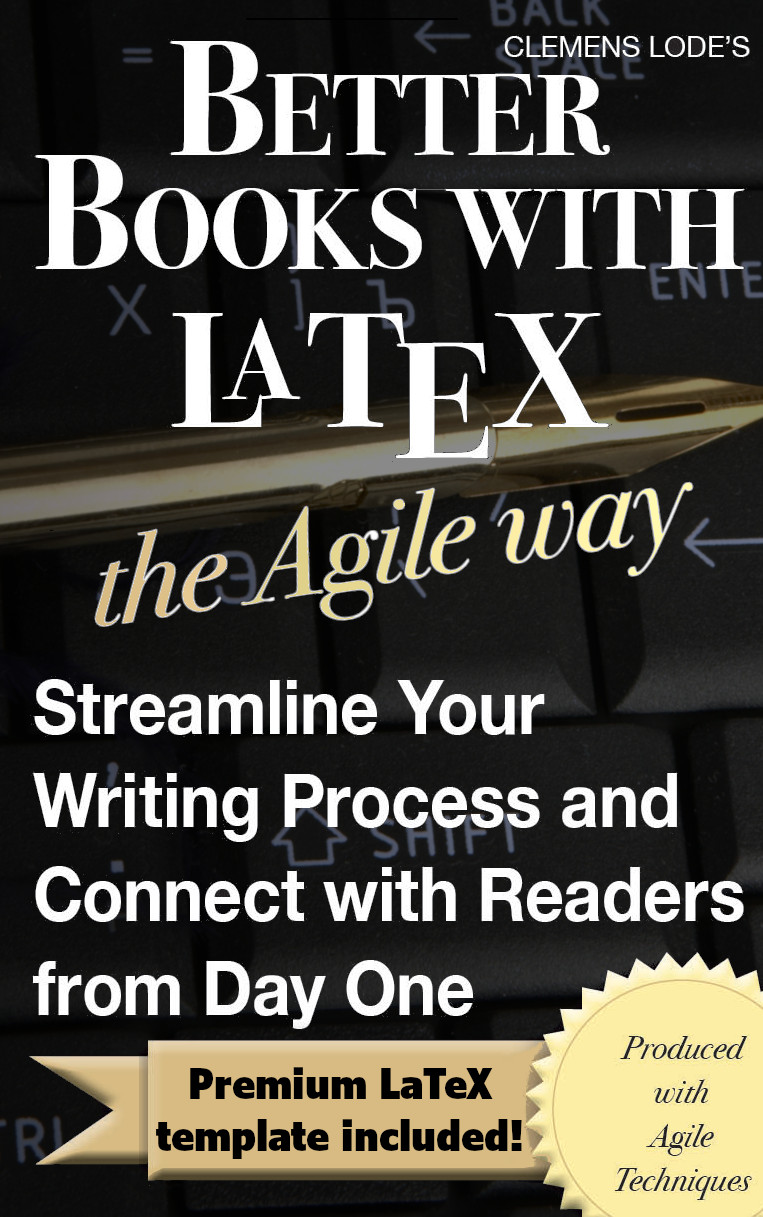
\includegraphics{images/cover.jpg}
	\caption{The cover of this book.}\label{fig:c1_cover}
\end{figure}

In \Cref{fig:c1_cover}, you can see the result of the command. Instead of
graphics, you can also include other TEX files that contain graphics (or
commands to draw graphics, see \Cref{sec:c1_tikzgraphics}).


\section{TikZ Graphics}\label{sec:c1_tikzgraphics}

For graphics, you can use the inbuilt TikZ graphics generator. Due to its
flexibility, I even recommend images you already have for a number of reasons:

\begin{itemize}
    \item TikZ graphics can very easily changed (especially for for example
    translations or making corrections).
    \item TikZ graphics are small and flexible. They can be easily scaled to any
    size and are directly integrated into your project (no time-consuming
    editing in an external graphics program necessary).
    \item TikZ graphics look better. As vector graphics are sent directly to the
    printer, we need not to worry about readability.
\end{itemize}

If you want to create a TikZ graphic, simply create a new TEX file in the
\textit{tex-images} folder and include it with \lstinline[language=Tex]!\input{...}! % chktex 27
(replacing \lstinline[language=Tex]!\includegraphics{}!) where you want to. 

Then, do a ``recompile from scratch'' by clicking on the top right corner of the
preview window (showing Warning or Error) to regenerate the TikZ file. If
``up-to-date and saved'' is shown, delete the \textit{tikz-cache} directory and
recreate it. 

For the format of the file itself, it is a series of commands surrounded by the
\lstinline[language=Tex]!\begin{tikzpicture}...\end{tikzpicture}!%
environment. Discussing all the commands is beyond the scope of this book, so I recommend three options:

\begin{itemize}
    \item Check out the PGF manual at \url{https://www.ctan.org/pkg/pgf}. It is
    more than 1100 pages full with documentation of each command and
    corresponding examples.
    \item Check out the few example TikZ pictures from my two books~\cite{PFH1E, PFH2E} in the \textit{tex-images} directory.
\end{itemize}

\chapter{Replace with Third Chapter Name} \label{c3_thirdchapter:cha}

\begin{figure}
    \centering
    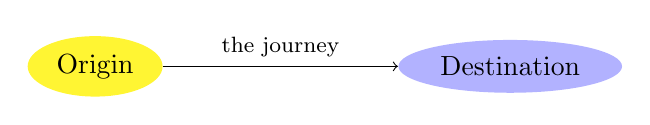
\begin{tikzpicture}
        \node[fill=yellow!80,ellipse] (origin) {Origin};
        \node[fill=blue!30,ellipse] (destination) at (15em,0) {Destination};
        \path (origin) edge[->] node[above,font=\footnotesize] {the journey}
        (destination);
    \end{tikzpicture}
    \caption{TikZ drawings will be output as SVG, which should be rendered by most modern browsers.}
\end{figure}

\begin{figure}
    \centering
    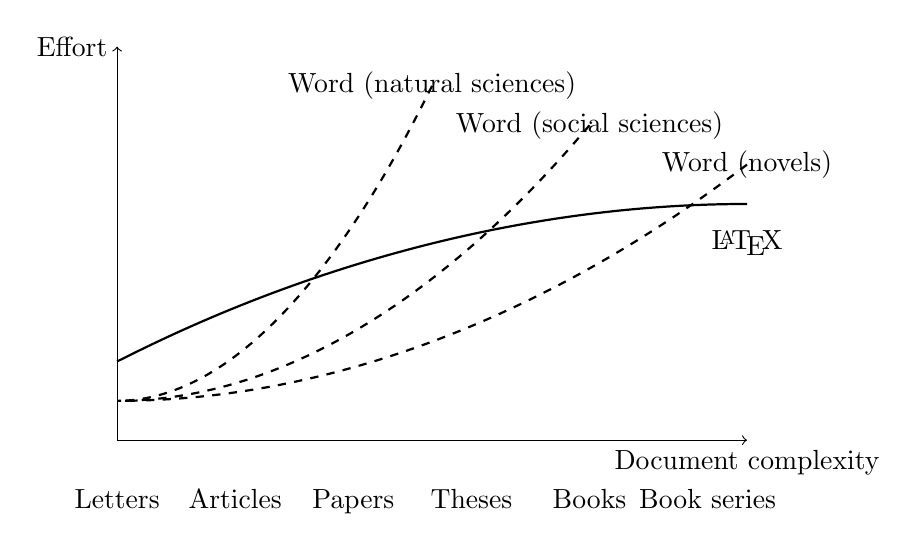
\begin{tikzpicture}

    % horizontal axis
    \draw[->] (0,0) -- (8,0) node[anchor=north] {Document complexity};
    \draw[->] (0,0) -- (0,5) node[anchor=east] {Effort};
    
    % labels
    \draw	(0,-0.5) node[anchor=north] {Letters}
    		(1.5,-0.5) node[anchor=north] {Articles}
    		(3,-0.5) node[anchor=north] {Papers}
    		(4.5,-0.5) node[anchor=north] {Theses}
    		(6,-0.5) node[anchor=north] {Books}
    		(7.5,-0.5) node[anchor=north] {Book series};
    
    \draw (8,3.5) node {Word (novels)};
    \draw (6,4) node {Word (social sciences)};
    \draw (4,4.5) node {Word (natural sciences)};
    \draw (8,2.5) node {\LaTeX{}};
    
    % Psis
    \draw[thick,dashed] (8,3.5) parabola[bend at end] (0,0.5);
    \draw[thick,dashed] (6,4) parabola[bend at end] (0,0.5);
    \draw[thick,dashed] (4,4.5) parabola[bend at end] (0,0.5);
    \draw[thick] (0,1) parabola[bend at end] (8,3);

\end{tikzpicture}
    \caption{Comparing complexity of \textit{Word} and \LaTeX{} depending on the application.}
\end{figure}

\begin{figure}
    \centering
    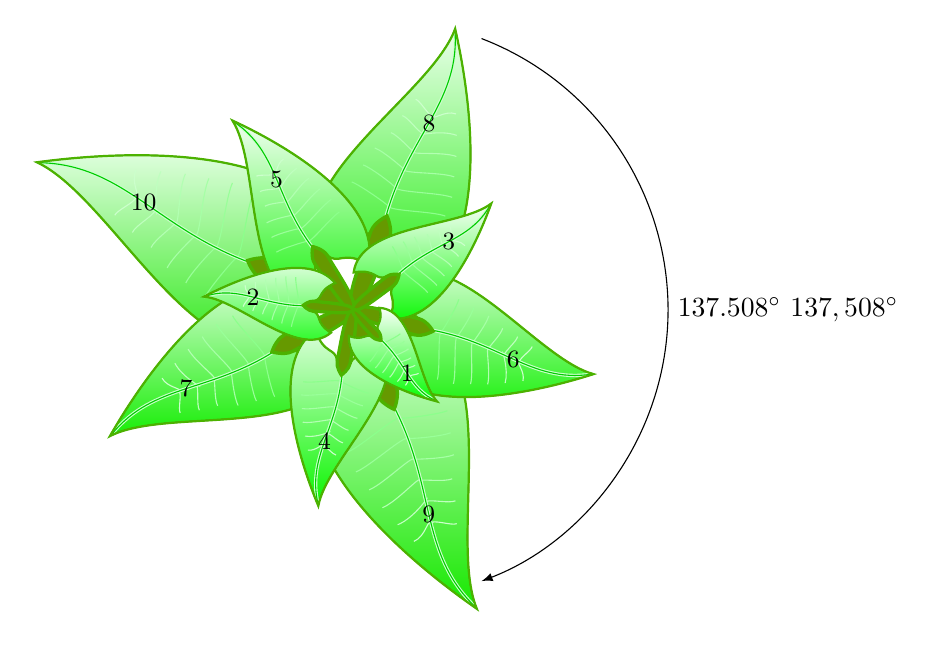
\begin{tikzpicture}
    \foreach \x in {10,...,1}
    {\draw[shade,bottom color=red!\x!green,top color=green!\x,x=0.3 pt,y=0.3 pt,scale={0.4+0.1*\x},rotate=222.5*\x] (0,0) .. 
    controls ( -11,  1) and ( -9, 50) .. (-10,80) ..
    controls ( -16, 60) and (-32, 75) .. (-50,40) .. 
    controls (-110,100) and (-0,230) ..  (  0,300)  node[below] (\x) {} ..
    controls (  45,230) and (110,100) .. ( 50,40) ..
    controls (  32, 75) and ( 16, 60) ..  ( 10,80) ..
    controls (   9, 50) and ( 11,  1) .. (  0,0) 
    -- cycle ;
    
    \draw[thin,green!45,x=0.3 pt,y=0.3 pt,scale={0.4+0.1*\x},rotate=222.5*\x] (-45,120) .. controls (-35,120) and (0,110) .. (-3,110) .. controls (0,105) and (40,120) .. (55,120);
    \draw[thin,green!40,x=0.3 pt,y=0.3 pt,scale={0.4+0.1*\x},rotate=222.5*\x] (-40,140) .. controls (-30,140) and (0,130) .. (-3,130) .. controls (0,125) and (40,140) .. (55,140);
    \draw[thin,green!35,x=0.3 pt,y=0.3 pt,scale={0.4+0.1*\x},rotate=222.5*\x] (-35,160) .. controls (-25,160) and (0,150) .. (0,150) .. controls (0,145) and (35,160) .. (50,160);
    \draw[thin,green!30,x=0.3 pt,y=0.3 pt,scale={0.4+0.1*\x},rotate=222.5*\x] (-25,180) .. controls (-17,180) and (0,170) .. (3,170) .. controls (0,165) and (30,180) .. (45,180);
    \draw[thin,green!25,x=0.3 pt,y=0.3 pt,scale={0.4+0.1*\x},rotate=222.5*\x] (-20,200) .. controls (-13,200) and (0,190) .. (6,190) .. controls (0,185) and (20,200) .. (38,200);
    \draw[thin,green!20,x=0.3 pt,y=0.3 pt,scale={0.4+0.1*\x},rotate=222.5*\x] (-13,220) .. controls (-8,220) and (3,210) .. (8,210) .. controls (10,205) and (18,220) .. (30,220);
    \draw[very thick,green!20,x=0.3 pt,y=0.3 pt,scale={0.4+0.1*\x},rotate=222.5*\x] (0,90) .. controls (-10,180) and (30,230) .. (1,297);
    \draw[thin,black!20!green,x=0.3 pt,y=0.3 pt,scale={0.4+0.1*\x},rotate=222.5*\x] (0,90)  .. controls (-10,180) and (30,230)  .. (1,297) node[midway,black] (num\x) {\small\x};
    \draw[very thick,red!30!green,fill=red!40!green,x=0.3 pt,y=0.3 pt,scale={0.4+0.1*\x},rotate=222.5*\x] 
    (0,0) .. 
    controls ( -11,  1) and ( -9, 50) ..
    (-10,80) .. 
    controls (-10,90) and (0,100) .. (0,100) ..
    controls (0,100) and (10,90) .. (10,80)..
    controls (   9, 50) and ( 11,  1) .. (  0,0) 
    -- cycle;
    \draw[thick,red!30!green,x=0.3 pt,y=0.3 pt,scale={0.4+0.1*\x},rotate=222.5*\x] (0,0) .. 
    controls ( -11,  1) and ( -9, 50) .. (-10,80) ..
    controls ( -16, 60) and (-32, 75) .. (-50,40) .. 
    controls (-110,100) and (-0,230) ..  (  0,300) ..
    controls (  45,230) and (110,100) .. ( 50,40) ..
    controls (  32, 75) and ( 16, 60) ..  ( 10,80) ..
    controls (   9, 50) and ( 11,  1) .. (  0,0) 
    -- cycle ;
    }
    \draw[->,>=latex,x=0.3 pt,y=0.3 pt,black] ([xshift=6pt] 8.east) arc (69:-69:350) node[midway,right] {$137.508^\circ$ $137,508^\circ$};
\end{tikzpicture}


    \caption{Example of a drawing made in TikZ.}
\end{figure}



\chapter{Introduction to micro-architectural attacks}
\label{chap:c7_cacheattacks}

Clementine Maurice, CNRS, IRISA\\
April 30, 2019 — Ben Gurion University, Israel

\section{Background \& Primitives} %arbel
\label{sec:BackgroundnPrimitives}

Micro-architectural side-channel attacks refers to a side-channel attack that exploit information leakage from the hardware infrastructure itself. The attacks can be found in a large scope on devices - servers, workstations, laptops, smart-phones, etc.

Normally, we assume a safe software infrastructure. Meaning that no software bugs, such as buffer overflow, is present. Nevertheless, such assumption does not imply safe execution, due to the fact that the information leaks because of the implementation, which is often driven by complex optimizations and design. Such leakages are not considered as 'mistakes' or 'bugs', but rather a trade-off decision between optimizing some aspects of the execution and potential information leakage.    

Potential outcomes of such attacks as described can be crypto primitives, which is common with other side-channel attacks, but also other sensitive information such as keystrokes and mouse movements.  

In terms of sources of leakage, we saw in previous chapters sources such as power consumption or electromagnetic leaks. However such sources are harder to come across by an attacker because they require physical proximity and access to the device, which is more typically to embedded devices. In our case we are only require that the attacker have somewhat remote access to the device, meaning that the attacker can run code on the hardware infrastructure of the machine. Such scenarios can be found in cloud providers renting computational resources to a costumer, Java-Script code running in a browser and others.

\subsection{Example: Cache attack on RSA Square-and-Multiply Exponentiation}
\label{subsec:CacheattackonRSA}

\begin{algorithm}
    \SetKwInOut{Input}{Input}
    \SetKwInOut{Output}{Output}
    \Input{base $b$, exponent $e$, modulus $n$}
    \Output{$b^e$ mod $n$}
    $X \leftarrow 1$
    \For{$i \leftarrow bitlen(e)$ \textbf{downto} $0$}
    {
    $X \leftarrow multiply(X,X)$
    \If{$e_i = 1$}
    {
    $X \leftarrow multiply(X,b)$
    }
    }
    \textbf{return} X
    \caption{Square-and-multiply exponentiation}
    \label{algo:SaM}
\end{algorithm}

Consider the binary exponentiation algorithm presented in Algorithm \ref{algo:SaM}. Notice that the execution flow of the algorithm relies heavily on the value of the bit $e_i$ of the private key. Now consider a scenario in which an attacker has information on the changes regarding the buffer holding the multiplier $b$. Such information can be considered as a query to the buffer and receiving as a result the latency of the query. If the buffer is in use, the query will be longer then if the buffer is unused.

\begin{figure}
    \centering
    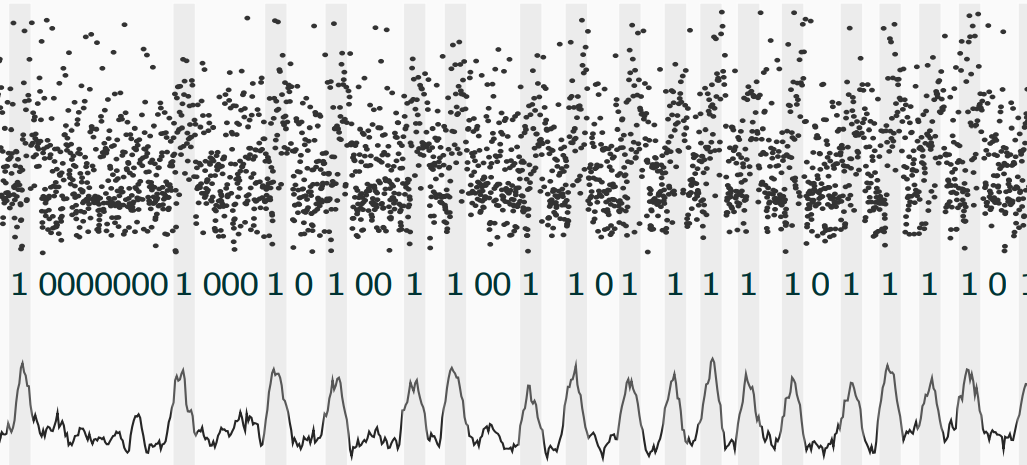
\includegraphics[width=\textwidth]{images/PPSM.PNG}
    \caption{Querying the buffer holding the multiplier $b$. The y axis is a latency scale, and the x axis represent the query index. The dotted plot is a scatter plot while the solid line is the normalized moving average.}
    \label{fig:PPSQ}
\end{figure}

In \Cref{fig:PPSQ} the resulting graph of the querying can be seen, in which the actual bits of the exponent can be clearly detected.

\subsection{Attack Model}
\label{subsec:attackmodel}
We assume that the attacker has no physical access to the device. Moreover, the attacker can only execute unprivileged code on the same machine as victim. Such scenarios in which this happens can be found, for example, when the victim install some malicious program on his machine/smartphone. Another examples can be found in could computing where an attacker has a victual machine on the same physical machine as the victim, or in a web environment in which the attacker runs unprivileged JavaScript code.

In the scope of this chapter we will focus on shared hardware in the form of data/instruction cache. While other shared hardware components can also include the DRAM and the memory bus (memory shared hardware) or the branch prediction unit and the arithmetic logic unit (CPU shared hardware), they are not in the scope of this chapter.

\subsection{Today's CPU Complexity}
\label{subsec:todaycpucomplex}
From 2012 onwards Intel has released a new family of microprocessors every year. Each comes with its own new microarchitectural schemes with new Characteristics. To gain performance upgrade in each new installment, that has on average 5\% increase in performance depending on the feature, very small optimizations, such as caches and branch prediction units are added. Such optimizations are the main reason for a side-channel information leakage to exist. Unfortunately, said optimization often come with no documentation since this is Intel intellectual property. Such lack in documentation makes it harder for an attacker to perform said side-channel attacks.

To emphasize today's CPU complexity, it is said that ``Intel x86 documentation has more pages than the 6502 has transistors" \cite{IntMan}, with 6502 being a reference to a 8-bit microprocessor, used in Apple II, Commodore 64, Atari 800 and more. It had, in the year 1975, roughly 3510 transistors, while the Intel Software Developer's Manuals is 4844 pages (may. 2018). In a more advance microprocessor, such as the 22-core Intel Xeon Broadwell-E5, more than 7 billion transistors can be found. 

\subsection{Background on Caches}
\label{subsec:backgroundoncaches}
In designing a cache side-channel attack, a proper understanding of how caches work, in great detail, is required. First, we need to acknowledge that the requirements for an 'ideal memory' oppose each other. Such requirements are zero latency, infinite capacity, zero cost and infinite bandwidth. The trade-offs are interconnect: \textbf{Bigger is Slower} - Bigger memory often comes with higher latency, due to the fact the it would take longer to determine the location to retrieve.  \textbf{Faster is Expensive} - A reduction in latency often means that a more expensive technology a needed. For example, SRAM is faster than DRAM, which in turn is faster than Disk memory. However, their cost ratio is the other way around. \textbf{Bandwidth is Expensive} - A wider bandwidth needs to come with additional banks, ports, higher frequency or faster technology. 

In our need to understand the use of caches, we need to examine the different memory technologies and why they are used the way they do. \textbf{DRAM} - Dynamic Random Access Memory is the technology that is often used as the main memory (or RAM), while \textbf{SRAM} - Static Random Access Memory is the technology used in caches. The DRAM latency is higher than the SRAM latency, but is cheaper to make. The main difference in cost arises from the fact that DRAM consist only of one transistor and one capacitor per cell, while the SRAM consist of six transistors per cell. Said difference also mean that DRAM is more dense. Finally, the DRAM cell layout and technology requires to periodically refresh each cell.

Since having Both a large and fast, single level of memory is unlikely, CPU's today are made with multiple levels of storage. The main idea is that progressively bigger and slower storage units are located in higher levels of memory, which are farther from the processor. The motivation for such design is to ensure that most of the data the processor needs is kept in the closer and faster levels.

\begin{figure}
    \centering
    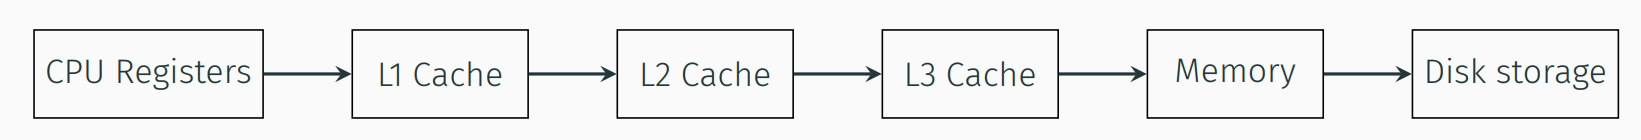
\includegraphics[width=\textwidth]{images/MemHier.PNG}
    \caption{Memory Hierarchy of a common CPU.}
    \label{fig:MemHier}
\end{figure}

The memory hierarchy can be seen in \Cref{fig:MemHier}, where data can reside in, at a given point in time, in the following storage units - in CPU registers, the different levels of the CPU cache, main memory or disk memory. 

\subsection{Caching Basics}
\label{subsec:cachingbasics}
The two main idea of caching is to exploit temporal and spatial locality. \textbf{Temporal Locality} is the notion that a program tends to reference the same memory location many times within a small window of time (for example, loops). The anticipation of such thinking is that recently accessed data will be accessed again soon. Therefor, a good strategy will be to store recently accessed data in automatically managed fast memory. \textbf{Spatial Locality} is the notion that a program tends to reference a cluster of memory locations at a time (for example, sequential instruction access or array traversal). The anticipation will be that surrounding of some accessed data will be accessed soon. A good strategy will consider storing addresses adjacent to the recently accessed one in an automatically managed fast memory. In detail, we want to logically divide memory into equal size blocks (lines) and fetch to cache the accessed block in its entirety.   

Moreover, there are two approaches to the management scheme, manual and automatic. \textbf{Manual Management} means that the programmer manages data movement across levels, which is not scalable for substantial programs. However, it is sometimes used in some embedded systems. \textbf{Automatic management} refer to a scheme in which the hardware itself manages data movement across the different levels in a way that is transparent to the programmer. Meaning that the average programmer does not need to know anything related to the memory hierarchy levels to write a program. On the down side, which begs the question on how to write a fast program if the management is automatic, in addition to what kind of side-channels could arise from such scenario.

The basic unit of storage in the cache is called a block or a line. The main memory is logically divided into cache blocks that map to locations in the cache. And when data is referenced, two outcomes can come of such action - a cache hit or a cache miss. A \textbf{Cache Hit} occurs when a line is referenced and is in the cache. The cached data will be retrieved instead of accessing main memory.  A \textbf{Cache Miss} occurs when a line is referenced and is not in the cache. The data will be fetched from main memory, passing though the cache, possibly eviction other data to ensure enough storage.

When designing a cache, we are faced with a number of design decisions to handle. \textbf{Placement}  - Essentially the place in which we will place or find a block in the cache. \textbf{Replacement} - We need often to remove data from the cache to make room for newer data. Which begs the question of what data to evict. \textbf{Granularity of Management} - The basic units of storage in different levels. Do we store the same amount of blocks across different levels or do we uniformly store the same size of blocks. \textbf{Write Policy} - When a write is being made, we need to decide whether to preform the write operation in all levels or passing the write data to a lower level only upon eviction from that level. \textbf{Instruction/Data} - When a program is executing, the instructions that are in need to be executed are required to be fetched from memory as well. The designer needs to decide whether to treat instruction and data memory as two separate  types or as one of the same.


\subsection{Set-Associative Caches}
\label{subsec:setassoccaches}

We will be focusing on a cache design that is often used in today's CPUs, which is set-associative caches. Which means that the cache will be logically divided into \textbf{Cache Sets}, which will be divided into \textbf{Cache Ways}. Each way will store a cache line worth of data. The division of the memory into different cache sets will be a direct mapping from the memory address. Namely, each address will be associated with a cache set according to a group of bits in the address which will represent the cache set index. The specific way in which the line will is to be fetch will be determine according to the cache replacement policy, since the cache set is expected to be full.  An
abstraction can be seen in \Cref{fig:SetWay}


\begin{figure}
    \centering
    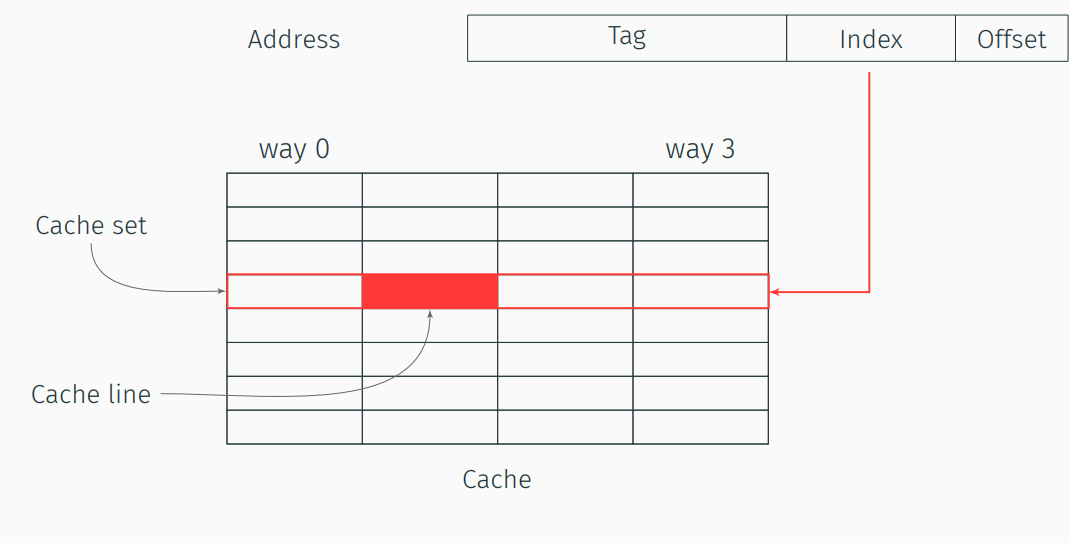
\includegraphics[width=\textwidth]{images/SetWay.PNG}
    \caption{Set-Associative Cache - The set index of a line derives from the set index bits of the address. The cache way is determine according to the cache replacement policy.}
    \label{fig:SetWay}
\end{figure}

Consider the following example: The cache has 8B cache lines, 16 cache sets each consisting of 2 ways. We can compute the set index of the address $(1011111110)_b$ by only looking at bits $b_3, b_4, b_5, b_6$, since we have 16 cache sets (4 bits) and 8 different cache line offset (bits $b_0, b_1, b_2$). Hence the cache set will be $(1111)_b$. We can also compute the size of the whole cache by multiplying the cache dimensions $8 \times 16 \times 2 = 256 $B.

\subsection{Virtual Addresses or Physical Addresses}
\label{subsec:addrorphysicaladdr}
Since we need the bits of address to determine its cache set, we are face with a problem due to the fact that programs running are only aware to the virtual addresses while the hardware side is aware to the physical addresses. The translation between virtual addresses and physical addresses is the responsibility of the MMU (Memory Management Unit).

There are four major ways of implementing such cache mapping according to the addresses. \textbf{VIVT} - Virtually-Indexed, virtually-Tagged. Meaning that there is no need to translate the addresses in order to know the mapping of the addresses into the cache, which is faster. On the other hand, such implementation causes aliasing issues as same virtual address maps to several different physical addresses. This aliasing is due to the tag not being unique, and will force a flush action to the entire cache on context swiching. \textbf{VIPT} - Virtually-Indexed, Physically-Tagged. Meaning that there will be a need for TLB translation for the tag, but can be looked up in parallel. Such mapping can be quiet fast. Moreover, if the set index bits are derived from the page offset, there is no aliasing, but the cache size is limited to the page size multiply by the number of cache sets. VIPT is used in Intel's L1 caches, with the default page size being 4K and each cache line is 64B, resulting in no larger than $2^6 = 64$ sets. \textbf{PIPT} - Physically-Indexed, Physically-Tagged. Meaning that the translation between virtual and physical addresses will have to be preformed, taking up time. On the other hand, no aliasing issues occurs and no required  limitation on the number of sets is present. Typically used in the larger Intel caches - L2 and L3. \textbf{PIVT} - Physically-Indexed, Virtually-Tagged. Meaning that all the limitations of previous ways apply, and is rarely used in practice. 

\subsection{Replacement Policy} 
\label{subsec:replacementpolicy}
We need to decide on a policy according to which a cache line will be evicted in order to make room for incoming data. Many replacement policies exist, namely FIFO (first in, first out), LRU (least recently used), LFU (least frequently used), random, a hybrid and more.

Intel commonly applies a LRU policy or a pseudo-LRU policy (since pure LRU is complex to implement). Which determines that the oldest cache line to be referenced will be evicted, As if each cache line is attached with a time-stamp that is updated on access. An example can be thought of by having $n$ way cache set and $n+1$ different lines of memory that are mapped into said cache set and are accessed in order. The first $1,\dots,n$ lines will fill the cache ways, while the $n+1$ access will evict the first memory line from the set, since all the set ways are full.  

A potential issue arises with LRU policy when a program need to access cyclically $n+1$ memory lines (``program working set") that are mapped to the same $n$ way cache set. This is referenced as a 'set thrasing' and will result in $0\%$ hit rate. If we compare LRU policy to a random policy, depending on the workload, some studies have shown that LRU and random replacement policies have the same hit rate on average.

When implementing a cache side-channel attack, we will normally will want to evict some special memory location from the cache. Considering a non-LRU replacement policy will mean that evicting a memory line from the cache will not necessarily be practical, since there is no guaranty that if the attacker access memory locations in a specific pattern we will evict the whole set from the cache. 
\subsection{Caches on Intel CPUs}
\label{subsec:cachesonintelcpus}
\begin{figure}
    \centering
    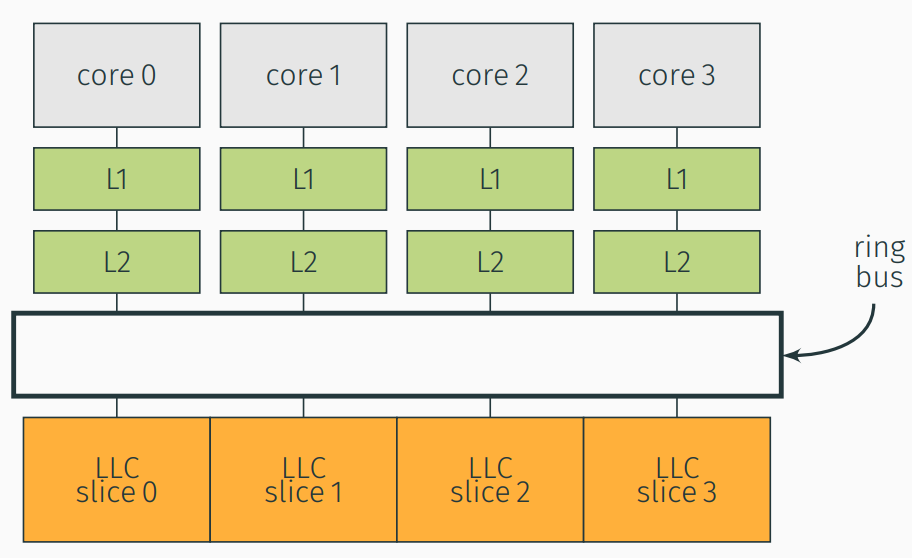
\includegraphics[width=\textwidth]{images/IntelCPU.PNG}
    \caption{Basic Intel CPU - each core has its own L1 and L2 caches, while all connected to a larger sliced L3 cache which can be accessed from all cores. }
    \label{fig:IntelCPU}
\end{figure}

In \Cref{fig:IntelCPU} we can see an abstraction of an Intel CPU architecture, on which every core has its own dedicated L1 instruction and data cache, in addition to a slightly bigger L2. All cores are connected via an interconnected bus to the last level cache (LLC/L3). The LLC often is sliced intro the number of cores, having a dedicated slice to each core, while having all cores being able to access all slices. The common practice is that the different levels of caches are inclusive, meaning that a lower level cache is a super-set of the higher ones.  

In order to preform a cache side-channel attack, an attacker can optimize its cache usage, among other things, using the following command: \texttt{prefetch} - A suggestion to the CPU that some memory line will be accessed soon, can trigger fetching that line into the cache by the CPU. \texttt{clflush} - Cache line flush, instructs the CPU to flush a memory line from all levels of the cache. The two instructions are based on virtual addressed.

The different latencies of the different cache levels, as well as the timing difference between a cache miss and a cache hit, as can be seen in \Cref{fig:cache_hits_misses_hist}, are the main primitives of most cache side-channel attacks that will be discussed by the end of this chapter.  

\section{Cache Attacks Techniques} %ben
\label{sec:cacheattackstech}

Microarchitectural attacks exploit hardware properties that allow inferring information on other processes running on the same system.
In particular, cache attacks exploit the measurable timing difference between the CPU cache and the main memory. They have been the most studied microarchitectural attacks for the past 20 years, and were found to be powerful to derive cryptographic secrets \cite{Percival2009}. In such attacks, the attacker monitors which memory lines are accessed, not the content of a certain memory line.

\noindent Cache attacks are being used in one of the two following common scenarios:
\begin{itemize}
\item \textbf{Covert channel}: two processes communicating with each other when they are not allowed to do so, e.g., across VMs.
\item \textbf{Side channel attack}: one malicious process spies on benign processes, e.g., steals crypto keys, spies on keystrokes etc. 
\end{itemize}
We will focus on side-channel attacks.

\subsection{Cache Side-Channel Timing Attacks}
\label{subsec:cachesidechanneltiming}
Every timing attack works by the following steps:
\begin{enumerate}
    \item Learn timing of different \textit{corner cases}.
    \item Recognizing these corner cases by timing only.
\end{enumerate}
Here, our corner cases are \textit{hits} and \textit{misses}.

\subsubsection{Building the Histogram}
\label{subsubsec:buildingthehistogram}
The first step towards the attack is to build the histogram of the corner cases, cache hits and cache misses. We measure the time for each case many times in order to get rid of noise. Thus, we have a histogram and we can find a threshold to distinguish the two cases.

\noindent Building the histogram for cache hits is done by the following loop:
\begin{enumerate}
    \item Measure time.
    \item Access variable (always cache hit).
    \item Measure time again.
    \item Update histogram with delta.
\end{enumerate}

\noindent Building the histogram for cache misses is done by the following loop:
\begin{enumerate}
    \item Flush variable (\texttt{clflush} instruction).
    \item Measure time.
    \item Access variable (always cache miss).
    \item Measure time again.
    \item Update histogram with delta.
\end{enumerate}

\noindent Having the two histograms, as in \Cref{fig:cache_hits_misses_hist}, we determine the threshold to be as high as possible such that there will be no cache miss below. 
\begin{figure}[!ht]
    \centering
    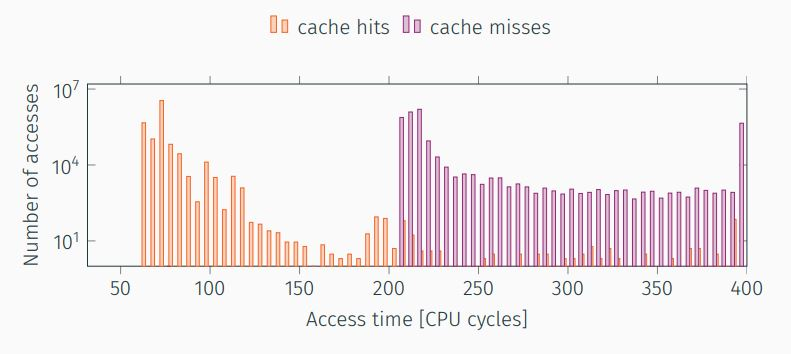
\includegraphics[width=\textwidth]{images/cache_hits_misses_hist.JPG}
    \caption{Timing differences histogram of cache hits and cache misses.}
    \label{fig:cache_hits_misses_hist}
\end{figure}

\subsubsection{How to Measure Time Accurately}
\label{subsubsec:howtomeasuretimeaccuractely}
Consider the fact that the time intervals of our cases is (relatively) very short timings, we ask how to measure time accurately. For such short timings, it is common to use the Time Stamp Counter (TSC) via the unprivileged \texttt{rdtsc} instruction as following:
$$[...] \rightarrow \texttt{rstsc} \rightarrow \mbox{function()} \rightarrow \texttt{rstsc} \rightarrow [...]$$
\noindent By using this instruction, due to out-of-execution, the actual execution order could be different, resulting with wrong measurements. The solution is to use the pseudo-serializing instruction \texttt{rdtscp} or to insert a serializing instruction like \texttt{cpuid} or use to fence instructions like \texttt{mfence} \cite{benchmark2010}.

We will now introduce two cache attack (main) techniques: Flush+Reload \cite{Gullasch:2011:CGB:2006077.2006784, Osvik:2006:CAC:2117739.2117741, Yarom2014} and Prime+Probe \cite{Percival2009,Osvik:2006:CAC:2117739.2117741,Liu:2015:LCS:2867539.2867673}. Both of them are exploitable on x86 and ARM and can be used for both covert channels and side-channel attacks.
\subsection{Flush+Reload}
\label{subsec:flushreload}
The attack is made of four basic steps and it goes as following:
\begin{enumerate}
    \item \textbf{Map. } The attacker maps a shared library (Illustration in \Cref{fig:fr_sharedlib}), by doing that he will have a shared cache line with the victim.
    \item \textbf{Flush.} The attacker \textit{flushes} the shared cache line, it can be done via unprivileged instruction like \texttt{clflush}.
    \item \textbf{Victim.} The attacker lets the victim load (or not load) the shared line, depending on the victim's behaviour.
    \item \textbf{Reload.} The attacker reloads the shared cache line. If the cache line has a \textit{hit} the attacker infers that the victim loaded the data on the previous step, if the cache line has a \textit{miss} the attacker infers that the victim did not load the data on the previous step.
\end{enumerate}

\begin{figure}[!ht]
    \centering
    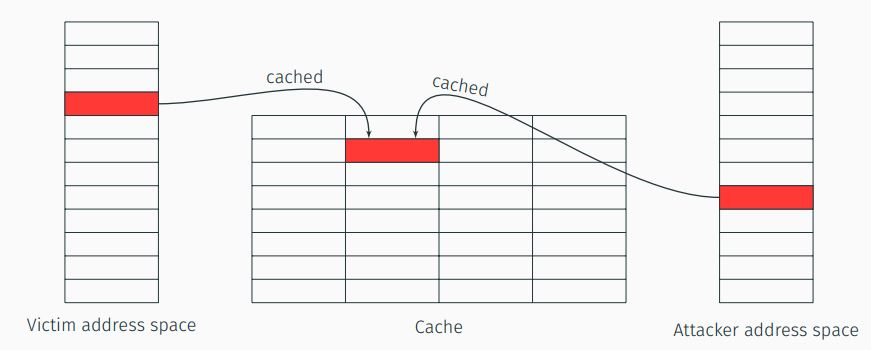
\includegraphics[width=\textwidth]{images/fr_sharedlib.JPG}
    \caption{Attacker maps shared library (shared memory, in cache), shared cache line marked in red}
    \label{fig:fr_sharedlib}
\end{figure}

\begin{figure}[!ht]
    \centering
    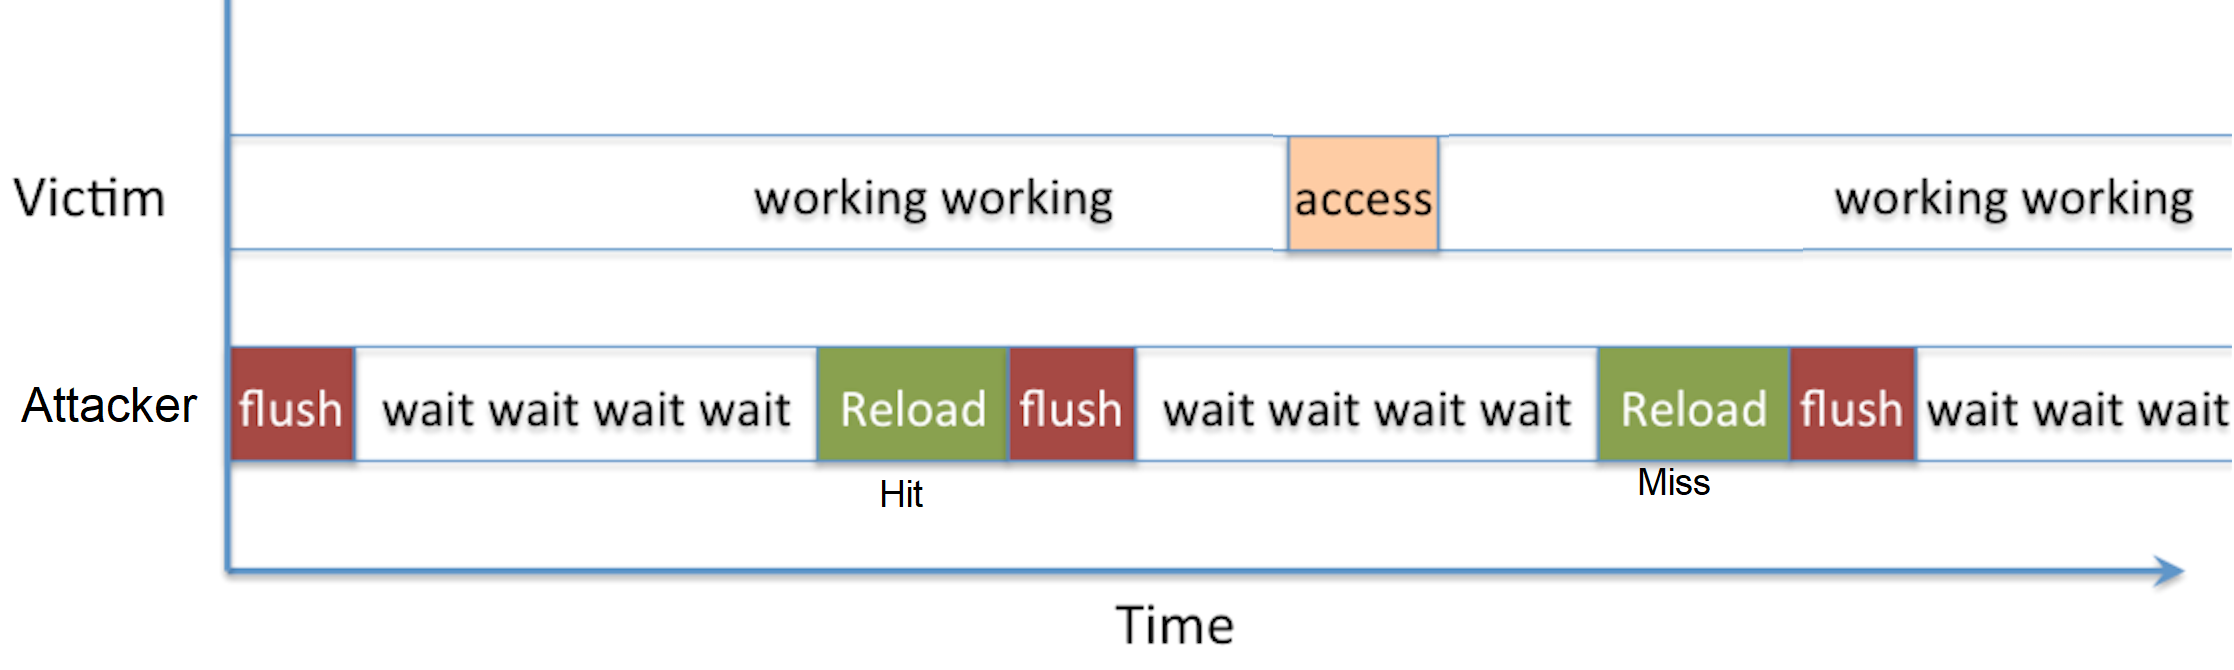
\includegraphics[width=\textwidth]{images/fr_flow.png}
    \caption{Flush+Reload attack flow. Between the first flush and the first reload the victim did not access the shared cache line, so the first reload resulted with a cache hit. Then, after the second flush the victim accessed the shared cache line and hence, the second reload resulted with a miss.}
    \label{fig:fr_flow}
\end{figure}

\noindent The first step (Mapping a shared library) can be done once, while steps 2-4 are repeatable as much as the attacker wants. The main advantage of this attack technique is the fine granularity, which is 1 memory line (usually 64B). On the other hand, this technique is somewhat restrictive, it needs \texttt{clflush} instruction, which is not always available e.g., on ARM-v7 and it needs a shared memory. Illustration of the attack flow in \Cref{fig:fr_flow}.

\subsubsection{Shared Memory}
\label{subsubsec:sharedmemory}
Common method to achieve a shared memory is by a feature called \textit{page-deduplication}. When two different independent processes are loading the same system library, some of their memory pages will be identical, when the operating system (in a cloud scenario - the hypervisor) identify separate identical physical memory pages, if page-deduplication is enabled, it will merge the physical pages in order to save physical memory, and two different virtual memory pages, one of each process, will be mapped into the same physical memory page. As of today, no cloud service company that takes itself seriously is using memory deduplication, e.g., Amazon EC2.

\subsection{Prime+Probe}
\label{subsec:primeprobe}
First, for the Prime+Probe attack to work, the Last-Level-Cache (LLC) should be inclusive, i.e., the LLC is a superset of the L1 cache and the L2 cache. Thus, data evicted from the LLC is also evicted from L1 and L2.
In inclusive caches, a core can evict lines in the private L1 of another core.
The attack is made of the three following steps:
\begin{enumerate}
    \item \textbf{Prime.} The attacker primes the cache by reading memory lines from its own exclusive memory (no shared memory).
    \item \textbf{Victim.} The attacker lets the victim evict (or not evict) lines while running, depending on the victim's behaviour.
    \item \textbf{Probe.} The attacker probes data in a similar way of the prime step but with measurement of how much time it takes to load the lines (Hit / Miss), for each cache set, the attacker determine if the cache set has been accessed.
\end{enumerate}

\begin{figure}[!ht]
    \centering
    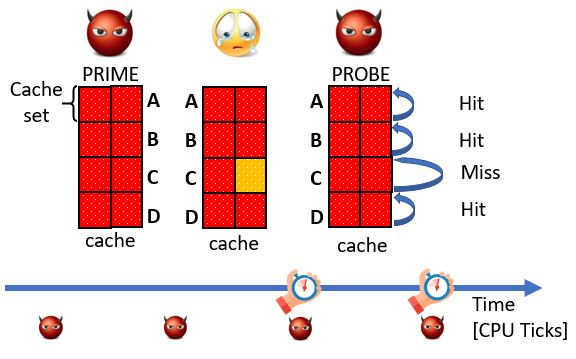
\includegraphics[width=\textwidth]{images/pp_flow.JPG}
    \caption{Prime+Probe flow.}
    \label{fig:pp_flow}
\end{figure}

\noindent In compare to Flush+Reload, this attack technique is less restrictive: it does not require \texttt{clflush}, does not assume shared memory and possible from JavaScript. On the other hand, the granularity is coarser: 1 set.  Illustration of the attack flow in \Cref{fig:pp_flow}.

In practice, we need to evict caches lines without \texttt{clflush} or shared memory, so the following questions arise:
\begin{itemize}
    \item Which addresses do we access to have congruent cache lines?
    \item How do we do that without any privilege?
    \item In which order do we need to access them?
\end{itemize}
For doing that, we need an \textit{eviction set}: addresses in the same set, in the same slice and an \textit{eviction strategy}.

\subsubsection{Eviction Set}
\label{subsubsec:evictionset}
\footnote{From now on, most of the details are correct for a common Intel CPU architecture.}
We want to target the L3 for cross-core attacks and we need addresses that have the same set index. Consider the following cache settings, L3 for a 2-core CPU: 4096 sets, 64B-lines, 12 or 16 ways. Since each memory address indicates one memory byte, the 6 least significant bits of the physical address indicate the line offset. For the sake of simplicity, we assume that the cache is not sliced, since there are $4096=2^{12}$ cache sets, the next 12 bits indicate the cache set. The L3 is physically indexed, so we need to choose addresses with fixed physical address bits. Unfortunately, address translation from virtual to physical is privileged. One of the properties of a virtual address is that a page offset stays the same from virtual to physical address, thus, some of the least significant bits of the virtual address can be used as a sneak peak to the physical address. A typical page size is 4KB, which means just 12 bits of page offset, i.e, 6 bits of line offset and 6 least significant bits of the cache set out of 12. To overcome this limitation, we can use a special type of enlarged pages called \textit{Huge Pages} which are 2MB size each, that is - 21 bits of page offset. This way the set index bits are included in the 21 LSB of the address.

We now have another issue, in practice, the L3 is divided in slices, as many slices as cores. We usually have 2048 sets per slice, that is, actually 11 bits for the set index. We cannot infer the slice number directly from the address, neither from the virtual or the physical. The slice number of each memory line is determined by a hash function which takes all the address bits as input, including physical page number bits (outside the known bits from page offset). Illustration of which bits of the address indicates what for both typical pages and huge pages is shown in \Cref{fig:slicedcache}.

\begin{figure}[!ht]
    \centering
    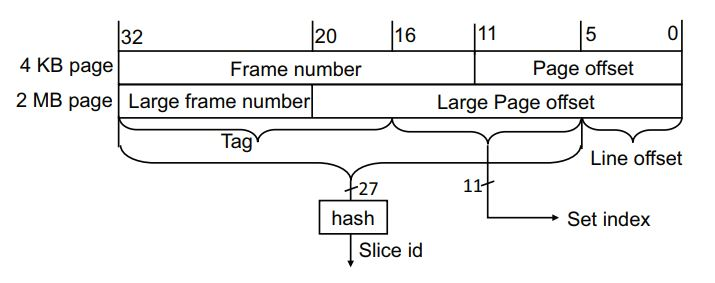
\includegraphics[width=\textwidth]{images/slicedcache.JPG}
    \caption{Sliced cache.}
    \label{fig:slicedcache}
\end{figure}

In addition, the mentioned hash function is undocumented, it designed for performance. But, it does not mean that it is impossible to target the same set in the same slice. Previous work \cite{EURECOM+4671} showed that the hash function can be reverse engineered, for example in \Cref{fig:hashfunc}.

\begin{figure}[!ht]
    \centering
    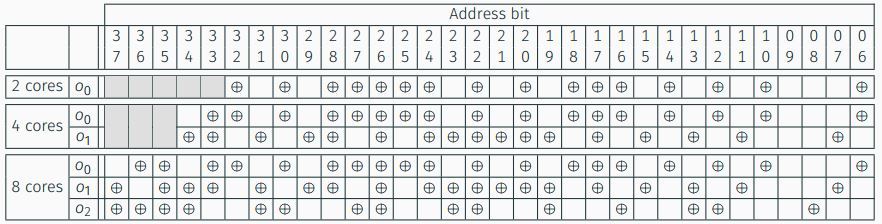
\includegraphics[width=\textwidth]{images/hashfunc.JPG}
    \caption{Three reversed engineered hash functions, depending on the number of cores. Function valid for Sandy Bridge, Ivy Bridge, Haswell, Broadwell}
    \label{fig:hashfunc}
\end{figure}

If the function is unknown, the process will be somewhat slower. But an eviction set can still be achieved via the following algorithm:
\begin{enumerate}
    \item Construct $S$, set of addresses with the same set index.
    \item Access reference address $x \in S$ (to load it in cache).
    \item Iteratively access all elements of $S$.
    \item Measure $t_1$, the time it takes to access $x$. it should be evicted.
    \item Select a random address $s$ from $S$ and remove it.
    \item Iteratively access all elements of $S$\textbackslash$s$.
    \item Measure $t_2$, the time it takes to access $x$ - is it evicted?
    \begin{itemize}
        \item If not, $s$ is part of the same set as $x$, place it back into $S$.
        \item If it was evicted, $s$ is not part of the same set as $x$, discard $s$.
    \end{itemize}
\end{enumerate}
\noindent Note that for a CPU with c cores: $16/c$ addresses in the same set and slice per 2MB page, we can apply the same algorithm with groups of addresses instead of single addresses and speed up the eviction set building process by up to three orders of magnitude.

\subsubsection{Eviction Strategy}
\label{subsubsec:EvictionStrategy}
In the Prime or the Probe step, the attacker evicts a cache set by filling it with $n$ addresses for a $n$-way cache. If the replacement policy is LRU, it access addresses from eviction set 1 by 1. If the replacement policy is not LRU, the eviction rate is lesser than $100\%$, e.g. $75\%$ on Haswell. For non-LRU caches, we can use some heuristics, as in \Cref{fig:haswellstrategy}, that will result with a higher eviction rate.

\begin{figure}[!ht]
    \centering
    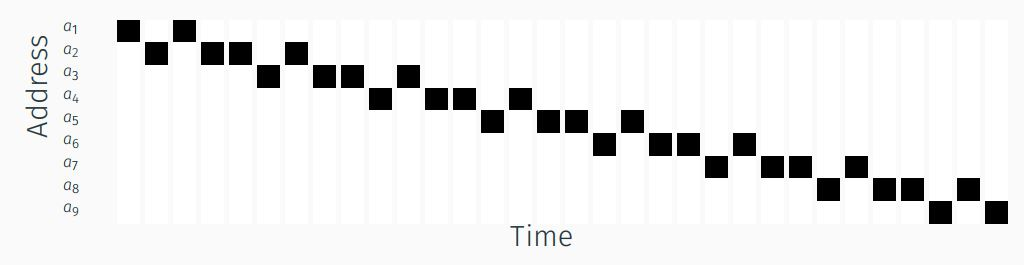
\includegraphics[width=\textwidth]{images/haswellstrategy.JPG}
    \caption{$a_1\dots a_9$ are in the same cache set. Fast and effective on Haswell: eviction rate $> 99.97\%$}
    \label{fig:haswellstrategy}
\end{figure}

\subsubsection{Conclusion}
\label{subsubsec:Conclusion}
To sum it up, in practice, for Prime+Probe on recent processors we need:
\begin{itemize}
    \item An eviction set, i.e., addresses in the same slice and with the same set index. Depends on the addressing.
    \item An eviction strategy, i.e., the order with which we access the eviction set. Depends on the replacement policy
\end{itemize}

\subsection{Hardware vs. implementations}
\label{subsec:Hardwarevsimplementations}

To perform a cache side-channel attack on some software you need two things: First, shared and vulnerable hardware. Note that there will be no side channel if every memory access takes the same time or if you cannot share the hardware component. Second, a vulnerable implementation. Note that a vulnerable implementation doesn't mean that the algorithm is vulnerable. For example, we can take specific implementation of AES and RSA, this doesn't mean that AES and RSA are broken. Not all implementations are created equal.

To sum up, hardware will most likely stay vulnerable, so patch implementations when you can. And remember, constant time is not enough - because an attacker can modify the internal state of the micro-architecture.

\section{Step by Step Attack Demo} %yaniv
\label{sec:stepbystepattack}

The target of the attack in this demonstration, is to get the timestamp of the keystrokes pressed by a user in a gedit program. We only target the timestamps and not the keystrokes themselves, as we are not able to fully recover the pressed keys.

The demonstration is performed on a non-virtualized Linux environment. A requirement to perform the attack is having an Intel CPU, as we need the inclusive property of L3 cache. The code for performing the attack can be cloned from the git repository \cite{GitClementine}. It is based on the Flush+Reload cache attack that we mentioned in \cref{subsec:flushreload} presented in \cite{Yarom2014} and \cite{Gruss2015}.

The attack is performed in 3 steps: calibration, profiling and exploit. For each of these steps, a folder exists in the repository.

\subsection{Step 1: Calibration}
\label{subsec:step1calibration}

In this step we want to create the histogram which depicts the cache misses and hits as a function of the number of CPU cycles. Then we will be able to extract the threshold that will match the CPU on which we perform the attack.
In order to perform the calibration, we run the following commands:

\begin{lstlisting}[language=bash]
  $ cd calibration
  $ make
  $ ./calibration
\end{lstlisting}

The calibration works by generating multiple cache misses and cache hits, and measuring the number of CPU cycles it takes to access a variable. Each of these cases is being performed multiple times in order to get rid of the noise.

\noindent We build a histogram of cache hits and cache misses as described in previous \cref{subsubsec:buildingthehistogram}. The output of the calibration program is a histogram of the cache misses and hits as shown in \Cref{fig:cache_hits_misses_hist}.

We can then find the threshold so it satisfies the following requirements:
\begin{enumerate}
    \item As high as possible
    \item Most cache hits are below it
    \item No cache miss below (we may see one exception due to the way the calibration is coded)
\end{enumerate}

For example, in \Cref{fig:cache_hits_misses_hist}, we can see that there is a clear line in approximately $220$ CPU cycles.

\subsection{Step 2: Profiling}
\label{subsec:step2profiling}

After finding the threshold, we can now profile in order to find the cache lines that are actually useful to get information about the target program. Choosing gedit as the target program, we first need to find the shared library that it uses, so we can give it as an input to the profiler. We then need to find this shared library file location and size. In order to do that, we can use the following one-liner:
\begin{lstlisting}
$ cat /proc/`ps -A | grep gedit | grep -oE "^[0-9]+"`/maps | grep r-x | grep libgedit
\end{lstlisting}
This is equivalent to first finding the pid with
\begin{lstlisting}[language=bash]
  $ ps -A | grep gedit
\end{lstlisting}
and then using this pid in
\begin{lstlisting}[language=bash]
  $ cat /proc/<pid>/maps | grep libgedit
\end{lstlisting}
then copying the line with r-xp permissions (x stands for executable).

Doing that gives the following line (memory range, access rights, offset, –, –, file name):

\begin{lstlisting}[language=bash]
7f2d83197000-7f2d8326d000 r-xp 00000000 08:02 1080575             /usr/lib/gedit/libgedit.so
\end{lstlisting}

Before we can feed the above line to the profiler, we need to update the threshold to the value we found in the calibration step. We can do this by editing the profiler source file (under the profiling directory) and updating the line with the constant 
\begin{lstlisting}[language=bash]
#define MIN_CACHE_MISS_CYCLES
\end{lstlisting}
to the threshold we have.

After updating the threshold, we can run \texttt{make} to compile the profiler. We then use \texttt{sleep 3} so we can have time to trigger the event before the profiler starts, and run the profiler with the line we found above: 
\begin{lstlisting}[language=bash]
sleep 3; ./profiling 200 7f2d83197000-7f2d8326d000 r-xp 00000000 08:02 1080575                    /usr/lib/gedit/libgedit.so
\end{lstlisting}

The profiler does its job by loading the shared library to its address space, and then doing flushes and reloads for each address in the address range given by the offset argument (0 in the above case), and the library size (1080575 bytes) for some given time (200 $\mu$sec for every address in the above command). The output is the number of hits that happened in every address.

The idea is that if a 0 is shown for a given address while triggering the event, then it means that the line in this address was never accessed for this event. Eventually, we will get lines with a number of cache hits, and we want the ones that have at least a non zero value when profiling.

\begin{figure}[!ht]
    \centering
    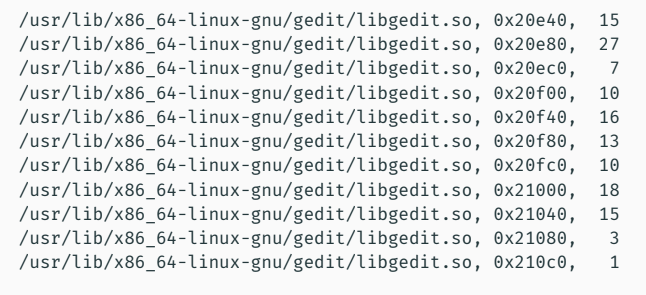
\includegraphics[width=\textwidth]{images/profiling-cache-hits.png}
    \caption{Addresses with cache hits.}
    \label{fig:profiling-cache-hits}
\end{figure}

Running the profiler with offset 0 while jamming a key, doesn't seem to generate cache hits, and we may only see 0. The reason for that, is that the code that handles keystrokes in the library is probably just not in the beginning of the library. Instead (and this is a cheat), we change the starting offset to 20000, and this is approximately where the code that handles keystrokes in the library is found. In real life we will have to wait until we get to something by running the template attack on the whole library. Running the profiler with this new offset, we can see in \Cref{fig:profiling-cache-hits} some addresses that have a non-zero value quite fast. The addresses with the high numbers are the ones we should further investigate in the exploit phase.

\subsection{Step 3: Exploitation}
\label{subsec:step3exploitation}

Equipped with the addresses from the previous step, we can now go to the exploitation dir, change the threshold constant (MIN\_CACHE\_MISS\_CYCLES) as we did for the profiler, and run \texttt{make}. Then we can run the program by 
\begin{lstlisting}[language=bash]
./spy <library-file> <offset>
\end{lstlisting}
giving one of the addresses we found as the offset argument. Starting from the address with the most hits, we can see that even if we are not pressing any key, we are still getting events. The reason for that is that this address is related to the blinking cursor. This is, of course, not really interesting information, and we can understand that it's not always the address that has the most hits that is the most valuable. Trying the next interesting address indeed gives us information about the pressed keys, which is what we wanted to achieve. However, moving the mouse also gives us a lot of hits, which is not perfect. What we will need to do is to inspect the addresses one by one until we find an address that will only work for keystrokes.

We can even further improve the attack by finding the complete matrix of the keystrokes for each of the keys as shown in \Cref{fig:cache-keymap-matrix}. We can see that for different keys, there is a different “signature” of the accessed addresses. Although we may not be able to identify each keystroke precisely, we can try to group the keystrokes to different addresses and eliminate some guesses if we are able to spy on more than one address at a time.

\begin{figure}[!ht]
    \centering
    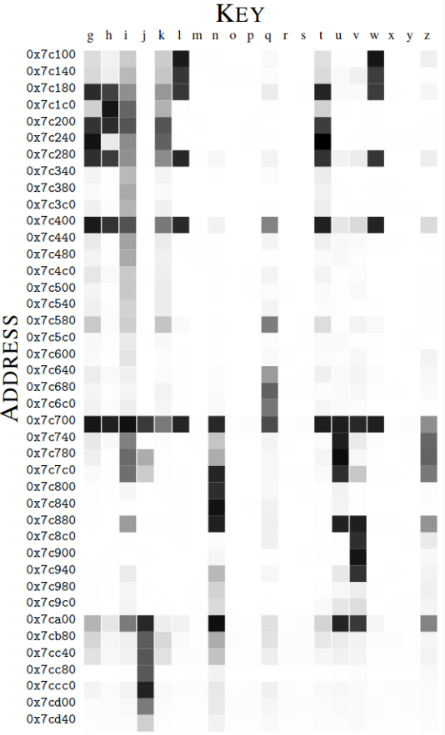
\includegraphics[width=0.8\textwidth]{images/cache-keymap-matrix.png}
    \caption{Complete matrix for each keystroke.}
    \label{fig:cache-keymap-matrix}
\end{figure}

Finally, as it may be annoying to perform the above process manually, we can automate the event triggering and other stuff as shown in \cite{GitGruss}.

\chapter{High Data Complexity Power/EM 1}\label{cha:High Data Complexity Power/EM 1}
So far, we've attacked two cryptographic systems in the course:
\begin{itemize}
\item RSA using Montgomery reduction with time as a side-channel
\item AES using simple power analysis
\end{itemize}
We attacked AES using simple power analysis, we had as an input a power trace consist of hundreds of thousands of points and then we actually wrote a classifier or let’s say dozen of classifiers and the classifier takes as input the power traces and outputs what is the hamming weight of the first byte of the state, and what was the hamming weight of the second byte of the state and so on… 
\begin{table}
\begin{center}
\begin{tabular}{ | c c | }
\hline
String & Hamming Weight \\ 
 \hline
 11101 & 4 \\ 
 \hline
 11101000 & 4 \\
 \hline
 00000000 & 0 \\
 \hline
 789012340567 & 10 \\
 \hline
\end{tabular}
\end{center}
\label{hammingWeights}
\caption{Hamming weights of different bit strings \cite{hamming}}
\end{table}

For AES you have 84 of this classifiers and we didn't actually talked about how these classifier are constructed but you can assume they take as input that power trace and output the hamming weight. 
A question arise: does the classifier look at the entire power trace? let’s say I have a classifier that wants to find out the hamming weight of the first sub-bytes operation of AES so you take the first byte of the plain text start with the first byte of the key and then you do sub bytes on this byte: you go to that sub bytes table and you replace the state with sub bytes of the state. 
Do you think that this classifier needs to look at the entire 1000 or 100,000 points of the trace? Or maybe it needs to look at the certain limited amount of points in the trace?
The answer is that our given power trace contains a lot of redundant information. We start our measurement a while before the first sub-byte operation happens, and therefore there are a lot of points in the data which is irrelevant for us (just an arbitrary operations that happened before the encryption started).

 So lets assume we have an army of classifiers, each one of these classifiers is going to be look at the certain points of the trace maybe 10 or 15 or hundred points in this very very large power traces. How can we know to find at which point to look at? We haven't taught that yet and we will go into that a little bit during this lecture. 
 
 Now, we want to combine the two attack methods: timing and simple power analysis and take the best part of each one of these methods combining them somehow and the results is going to be called differential power analysis.
 
 When we did a timing attack what was our threat model? What was the adversary allowed to do?
 We was allowed to send inputs to the device and get the outputs from the device and measure how long it took.
 
 We weren’t necessary in control of the inputs we just had to know when the input was provided we didn’t have to know what the input was. We just needed to know when was the input when was the output and find the time difference. We had to measure a lot of times and have many inputs, and then we did some statistics to analyze it.
  The various scenarios when we can justify a timing attack – when the device is in your position, or it's accessible across the web and so on.
  
  What about simple power analysis? What was the threat model there? What we allowed to do with the device?
  First of all we had to open the device and cut it power supply and connect a power probe which is the meter that measures the power consumption, this is an invasive attack so maybe it’s considered less probable that we actually allowed to do that as attackers. If you are doing an electromagnetic probe it would be less invasive but you still will have to get very close to the device, but it would be less detectable. 
  
  But what else we had to do before we perform simple power analysis? And now I’m reminding you what I just said couple of minutes ago, how do we actually do a simple power analysis, we have an army of classifiers, where this classifier came from? We need to train them. who do we train classifiers? we give them a lot of labeled data, we need to do what is called: \textit{profiling}, which means we have to get really good understanding of the DUT.
  How do we get this understanding? We have an offline phase.
  We have a device to which we can do reverse engineering and get really into it's internals. Maybe look at it with a microscope or we can understand completely how it works and then this device this similar to the DUT. The only things we're not allowed to know as adversary is the secret key.
  
  What is the difference between two devices? according to the Kirchhoff’s principles the difference between our DUT to what we use to learn is the \textit{current}. 
  
Now, one might ask: how do we get this copy of the device in the real world? well, we can buy it, we can steal it, maybe buy it online. you have to have a very involve offline phase before you can do a simple power analysis you have to get close to the device and do a reverse engineering if an justify it by buying stuff on eBay you can go to the trash you can look at the data sheets and so on.

Next thing in our attack is the \textit{online phase}.
In simple power analysis you can perform one or two simple measurements and what is the problem with these measurements  is that it's our only chance to measure and we have one trace that have to be very clean with very little noise. And of course, we can’t really control this noise. For example if we’re doing this outside the lab there’s going to be some kind of noise, but if we are using measurement equipment the measurement equipment is going to introduce noise to and the DUT is introducing noise by it self. Unfortunately, we can’t do so much about the noise in the simple power analysis scenario because we only have the online phase.

\subsubsection{What can we do if we had a little noise and we don't have the exact key?}
\textit{That's exactly our problem with simple power analysis}


Maybe only one byte is incorrect and we might try to search for the key around the guess? Let’s do a little bit of combinatorics: let’s say I got AES key which is 16 bytes long and it’s 8 bit implementation and I tried the key and it's wrong. 
Now, I’m trying to see if I change one byte in the key maybe that will fix the key. So, how many attempts well I have to perform? Lets try to change the byte with index 0 to all possible values, then change at index 1, then 2 and so it goes... 
How many decryptions should we do? We have 256 per position times the 16 bytes of the key. 
And if that didn’t work I didn’t find a key, maybe I’ll try 2 bytes combinations, so how many attempts I’ll have to do now? It’s 16 choose 2 which is more or less 16 squared so it’s two to the power of 4×2. So I chose to byte and then what I do is that I go over all the possible combination of this bytes which is two to the power of 16 so it is two to the power of 8+8=16. It grows up really fast and it’s going to be as bad as brute force pretty quickly. And what if I have to change tree bytes? it’s going up so I have to work very very hard if I don’t get the key right it blows up exponentially.
One might ask why we are talking about bytes and not bits? if we are looking at a 8 bit micro-controller a lot of the operations are going to be byte oriented so it’s going to be more likely to get the entire byte wrong. So if I don’t have the key right I am in trouble and I have to search and search very very hard. 

\textbf{The solution to this problem is to have a more complex offline phase which prepare us to the online phase.}

Simple power-analysis will work just fine if it's reasonable to conduct thousands of measurement on the same device in order to eliminate noise with statistics, however, it's not always practical.

\section{High Data Complexity Attacks}
(AKA: \textit{DPA} and \textit{CPA})

The main idea is to capture many traces and use statistics to recover the key.
The advantages of this methods are:
\begin{itemize}
\item Doesn't require detailed information about DUT (save us the cost of doing reverse engineering to the device)
\item Succeeds even under extreme noise
\end{itemize}
On the other hand, the drawback is that the attack model is different now, we need to own the device. That may cause some people to think that this attack model is irrelevant because it's not practical. In truth, it might be practical in a quite wide range of situations.
\subsubsection{Why would we want to get the secret of somebody else?}
A good example for it is how TV suppliers calculate your bill. You've a secret and you use it to identify yourself to the supplier. Based on that, the supplier should decide which TV shows you have access to, and how to charge you in case you watch paid TV shows, use VOD and etc... If someone get his hand on your password, he can use it to watch whatever TV shows he wants at whatever cost, because you're the one to pay the bill.
\subsection{How complex power analysis actually works}
Until now, we knew about 2 ways of attacking with side channel:
\begin{enumerate}
\item \textit{Timing Attack}
\item \textit{Simple power analysis}
\end{enumerate}
When we used timing attack, we tried many input, and the measurement for each input contained 1 output: for 1 input we had the time it took.
On the other hand, when we did Simple Power Analysis, for each input we had a huge power trace (vector of points which indicates the power consumption over time for a given input).
In other words, the data complexity was simple in both of these methods - we had a \(1d\) input.
Now we'll try to take it a step further and combine these methods and create a new method with \(2d\) input, which mean now we have high data complexity.
Instead of giving just the power trace, we'll give as an input the traces for various data at a fixated points in time. We have a set of data \({D_1, D_2, ..., D_n}\) and we have the power trace of the system for each one of these inputs, at the the time, i.e. the first point in the power trace for all these inputs, was taken at the same relative time.
So now our output isn't a vector but rather a Matrix \(M_{DxT}\).
\begin{figure}[H]
\centering
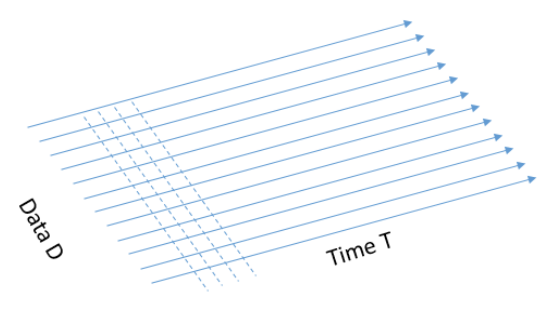
\includegraphics[width=0.8\textwidth]{images/Lecture6/DPA_Illustration.png}
\caption{many measurements over time}
\label{fig:DPA_Illustration}
\end{figure}

The suspicious reader should ask: how it's possible that we measure the power-traces of all the different data inputs all at the same time? That is indeed a challenge to align all the measurement along the time-line and some of the countermeasures to the attack we present here, will insert randomized operations or will change the clock speed so that we'll have trouble to align the power-traces along the time-line. If you're curious about that, you might find it interesting to look on the DPA book (the course book) and read about the countermeasures and the ways to overcome them.
\subsection{Using the Vaizata method}
The next thing we're going to do is to use the Vaizata similarly to how we did it with timing attacks. When we did timing attack, we made a guess about a bit of the key and then we measured how much time it took. Now, we're going to make an assumption that at sometime, the algorithm depends on the key, therefore the power consumption will be depended on the key. Finally we're going to check it with the measurements using some statistics. 

Unlike the timing attack where we knew that we measure the relevant data, when we used power analysis, we have a very long power trace where only few points relevant to us and all the other points represent data which isn't related to the key.

\begin{figure}[H]
\centering
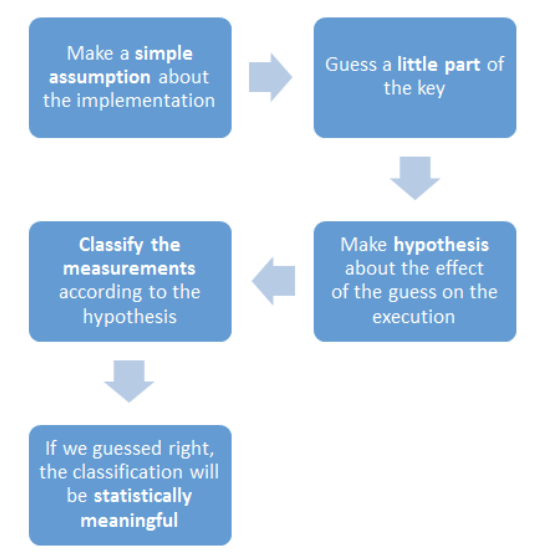
\includegraphics[height=0.9\textwidth]{images/Lecture6/vaizata.png}
\caption{Vaizata method stages}
\label{fig:vaizata}
\end{figure}

Now, we're looking for a stage during the AES algorithm, where a small amount of bits of the key, affect large amount of the bits in the state. The intuition here is that we want to find a stage in the algorithm, where the power consumption depends on the key value.

\begin{figure}[H]
\centering
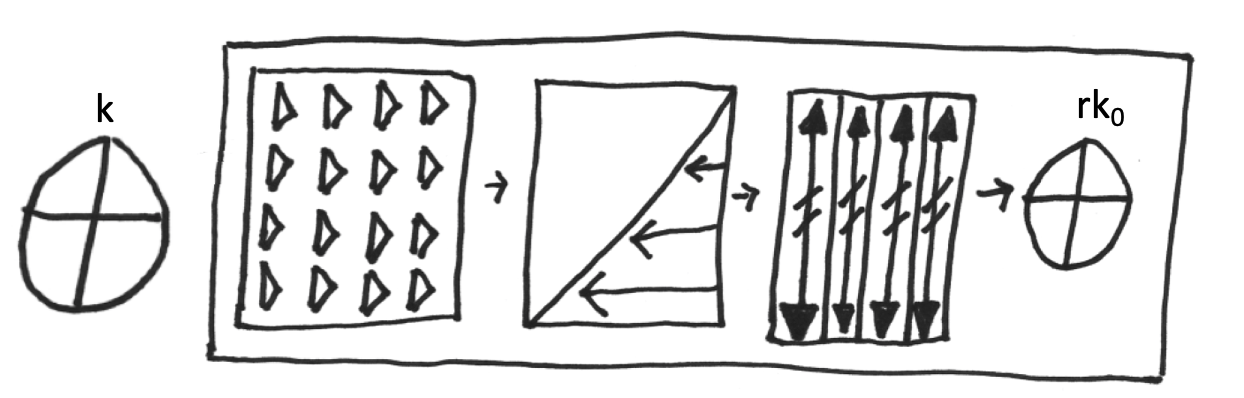
\includegraphics[width=0.8\textwidth]{images/Lecture6/AES-stages-figure.png}
\caption{AES stages}
\label{fig:aes-stages}
\end{figure}

We might consider measuring the power consumption just before the start of the algorithm, but in this case the key has no affect on the state. 
Next, we have the add round key. After this operation, each bit of the key affect exactly one bit of the state. Why is that? because we essentially "XOR" the key with the state, which so the the bit $k[0]$ affects the bit $s[0]$.

Our second operation will be the $subbytes$. The $subbytes$ operation is a value based substitution, where each possible state value is mapped to a different value as defined by the substitution matrix. In this stage, every bit of the key, affects 8 bits of the state! Why is that? if only one bit in the key was different, our add round key will cause another bit of the state to change, and that would lead the $subbytes$ look-up to bring an entirely different byte to the result state.

Next we have $shiftRows$, where still every bit of the key affects 8 bits of the state. Why is that? because we just moved the data, we didn't diffused it.

And now we have the $MixColumns$ operation. How many bits of the state now is affected by every bit of the key? In the $MixColumns$ operation, each byte depends upon 4 bytes, and each one of these 4 bytes are 8 bits that depends on the key. So we have now 32 bits of the state which is depends upon a single bit of the key.

As an attackers, we're going to focus on the point immediately after the $subbytes$ and right before the $shiftRows$. 

So based on this information, what should be our Vaizata assumption?
The assumption is that's the power consumption of the device is the function of the data so if we change the data, the power consumption changes. (A counter-measure for that will be to build a machine that consume the maximum power all the time).

Similarly to our attack on the RSA algorithm where we guessed a bit of the key, we're going now to guess a byte of the key (since AES is byte oriented). When we attacked RSA, we've splitted our data to 2 groups and then conducted $t-test$, but since we guess a byte, now we have a 256 groups. 

We know the value of the plaintext (it's given) and we're making a guess about the key, but how will we know the value of the $subbytes$? by Kerckhoffs's principle (which means that everything regarding the algorithm but the key is shared publicly).

So for each data point, and for each byte guesses, we have 256 options. 255 out of them will be meaningless and only one is the correct guess which should have statistic significance.

\begin{figure}[H]
\centering
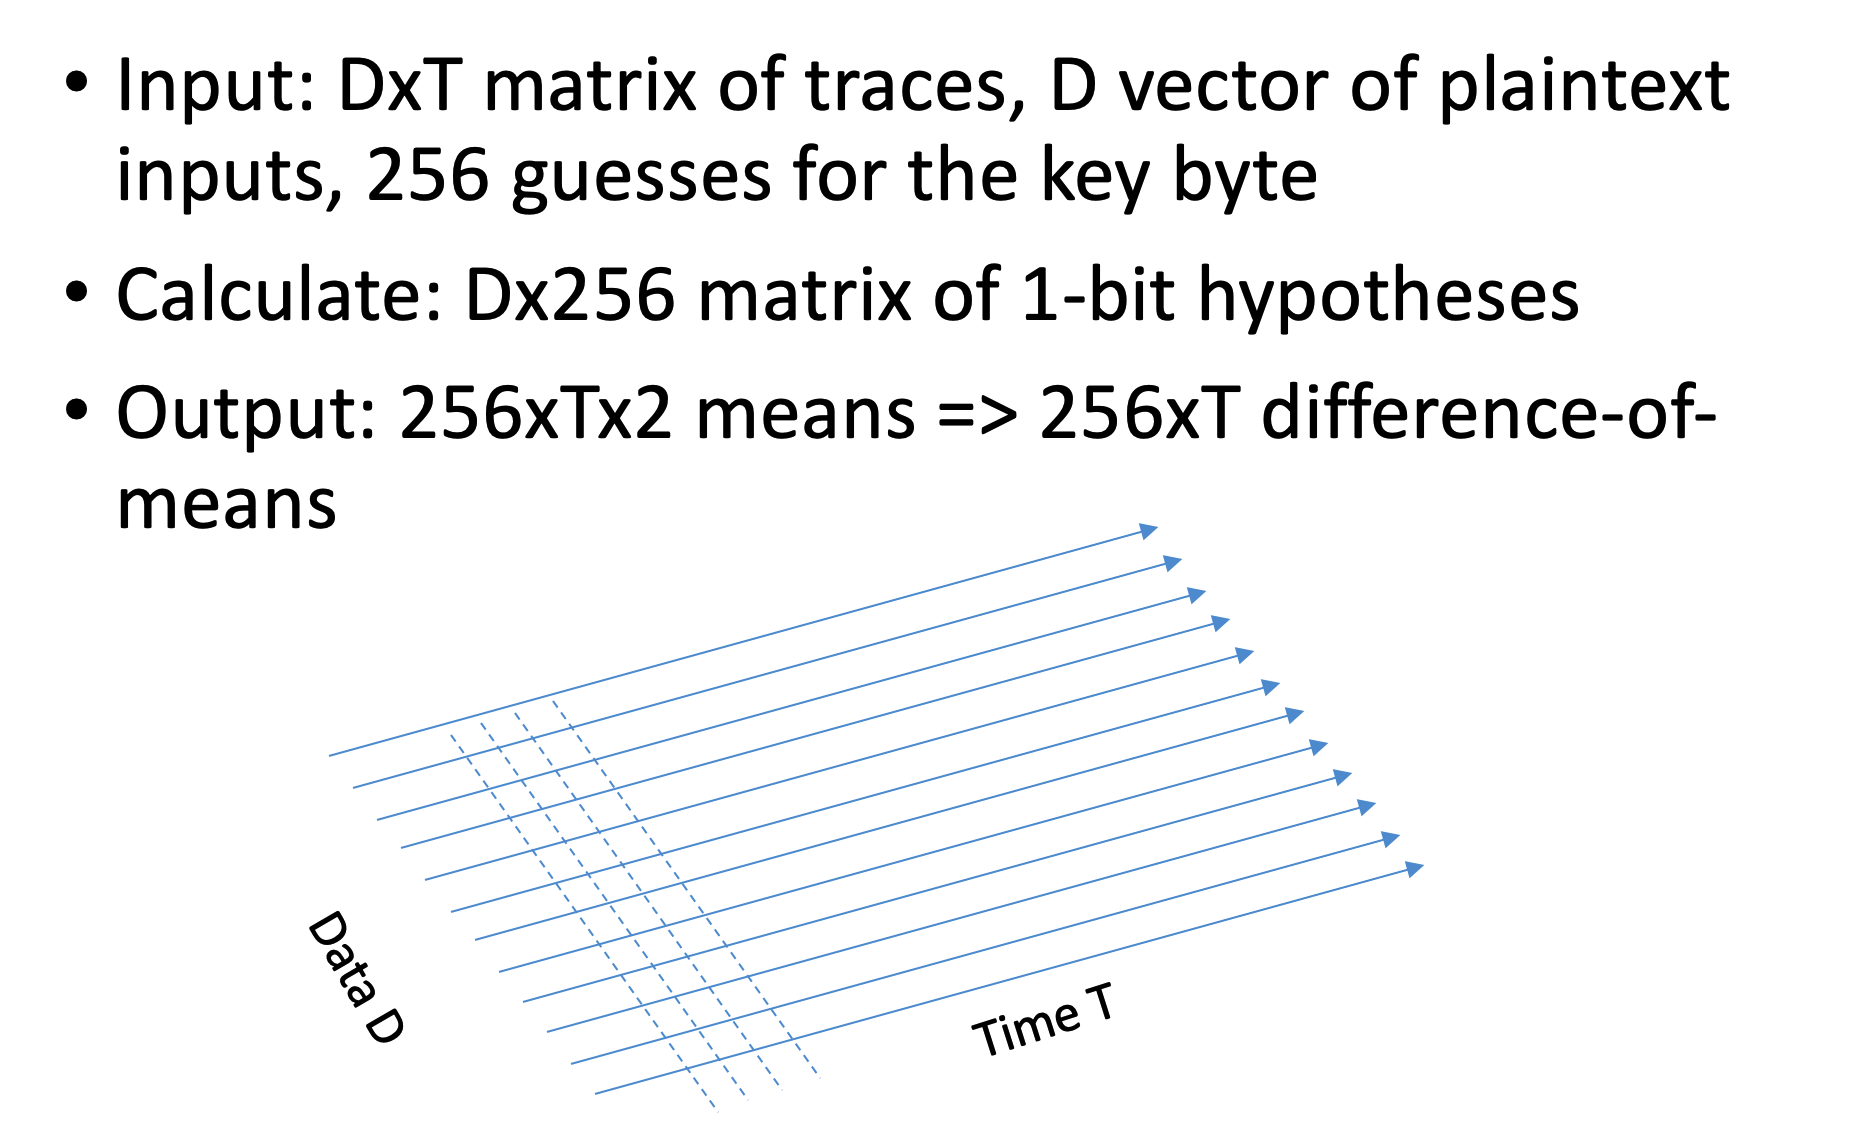
\includegraphics[width=0.8\textwidth]{images/Lecture6/dpa-separation-figure.png}
\caption{The way we separate the data to groups based on the guess}
\label{fig:dpa-separation-figure}
\end{figure}

The problem is that we have many different points on time, and we shall see a difference only at a certain point. Therefore what we do is as follows: for each guess, we split the measurements to 2 sets and we measure the difference between the means of their power traces on every point of time. At most of the points, the difference won't be significant, except to the point where the guess was done correctly. We illustrate it at figure \ref{fig:meansDiffFigure}.

\begin{figure}[H]
\centering
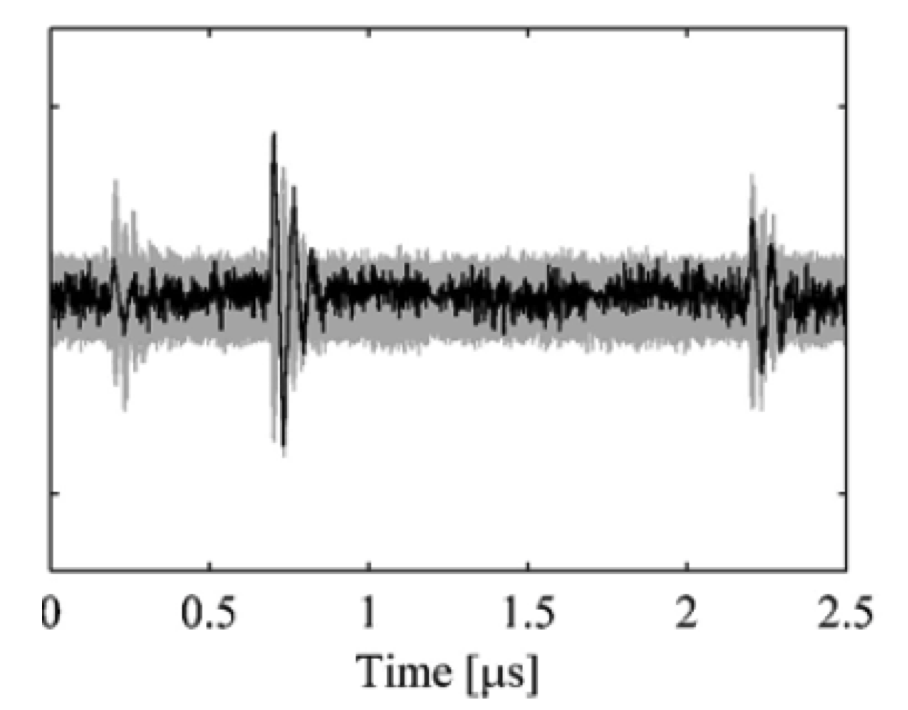
\includegraphics[width=0.8\textwidth]{images/Lecture6/meansDiffFigure.png}
\caption{the difference of means as a function of time}
\label{fig:meansDiffFigure}
\end{figure}

On the $X-axis$ we have the time and on the $Y-axis$ there's the difference of means. In Gray we can see the noise and even if we guessed the correct key we have a lot of similar points and that is because not all the times depends on the key. But we can see in the figure the moments of peak in the means difference, these moments are also called "the right times". These essentially should be the moments of the sub-bytes. If we incorrectly picked a peak which is a ghost noise, like in a point when we xor the plain the with the key, then we won't be able to find meaningful separation later on.

\section{DPA Lab}
In the class example, we attacked AES algorithm with 200 trace with size $30,000$ using an example data from the \textit{Power Analysis Attacks} book and we visualized the process.
First, we load the data and plot it in figure \ref{fig:traceByTime} with the following axes: $X-Axis$ will be the time and $Y-Axis$ will be the trace number. In addition, we had a dimension of color intensity which will be depend on the power consumption.
\begin{figure}[H]
\centering
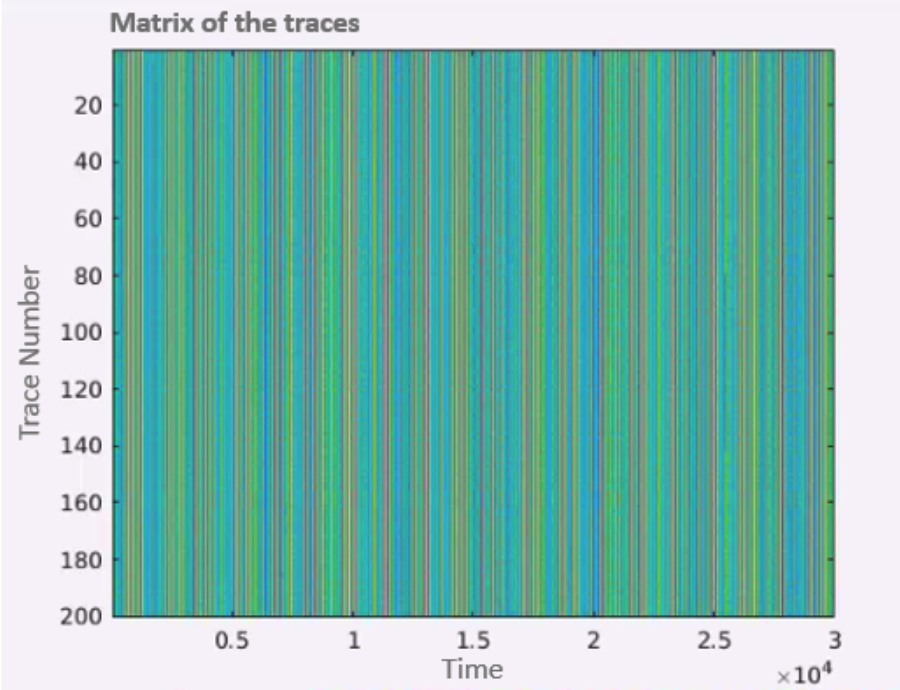
\includegraphics[width=0.8\textwidth]{images/Lecture6/traceByTime.png}
\caption{the traces' power consumption by time}
\label{fig:traceByTime}
\end{figure}
What we can see in plot \ref{fig:traceByTime} is that there are very aligned columns which indicate that the traces are aligned properly.
Our goal is to separate the power traces of the correct key from all the other traces. To do that, we start by showing in figure \ref{fig:2traces-by-time} by comparing the power consumption of 2 traces based on time.
\begin{figure}[H]
\centering
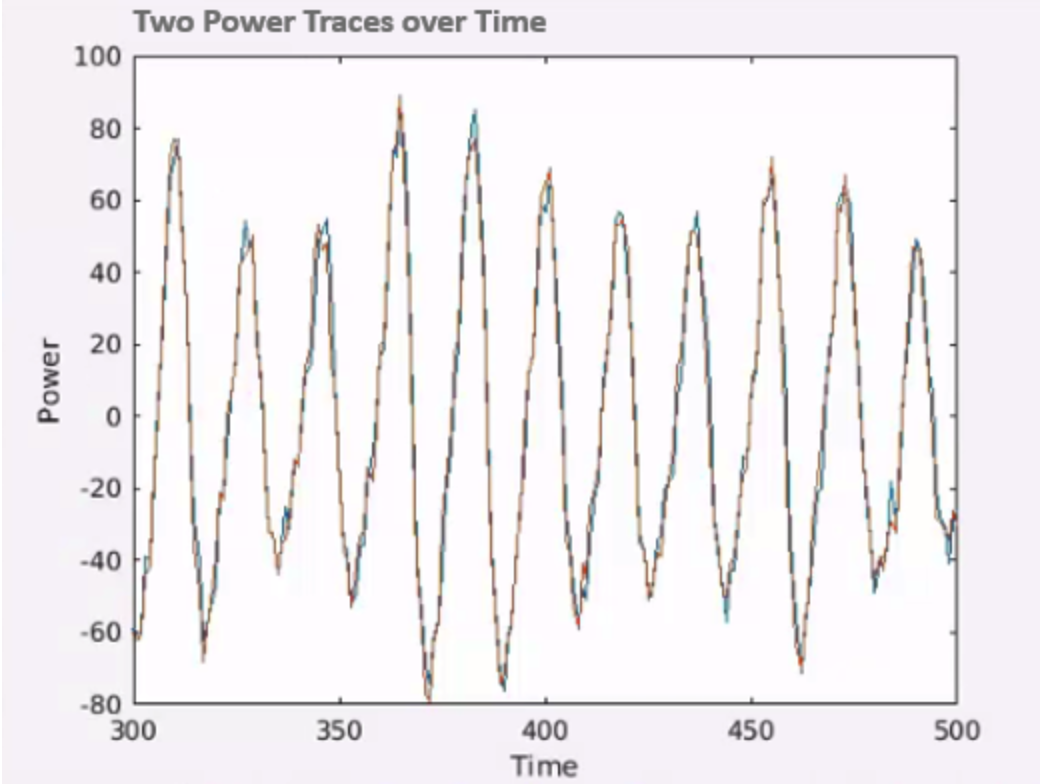
\includegraphics[width=0.8\textwidth]{images/Lecture6/2traces-by-time.png}
\caption{2 groups of traces by times}
\label{fig:2traces-by-time}
\end{figure}
We can see that both of them are overlapping, but if we had a difference between them we would be able to find a separations on this graph.

Therefore, in figure \ref{fig:intensity_by_guess} we test for each key guess and input, what was the power consumption, whereas yellow represent less power and blue more power.
\begin{figure}[H]
\centering
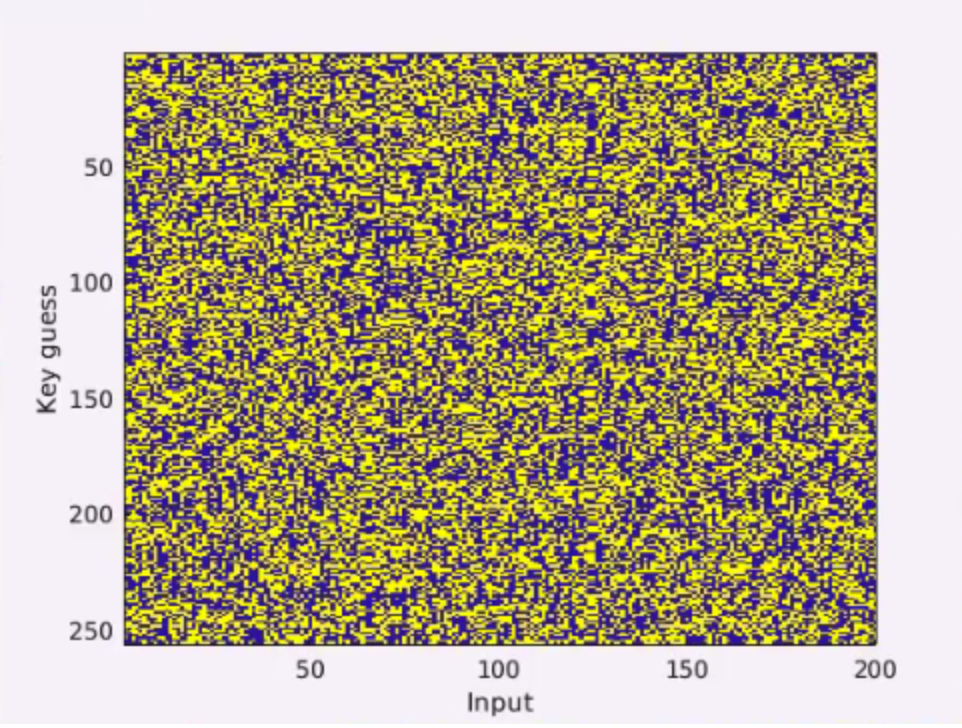
\includegraphics[width=0.8\textwidth]{images/Lecture6/intensity_by_guess.png}
\caption{power consumption by guess and input}
\label{fig:intensity_by_guess}
\end{figure}
Now we calculate the mean of power consumption for each guess and we plot if over time
\begin{figure}[H]
\centering
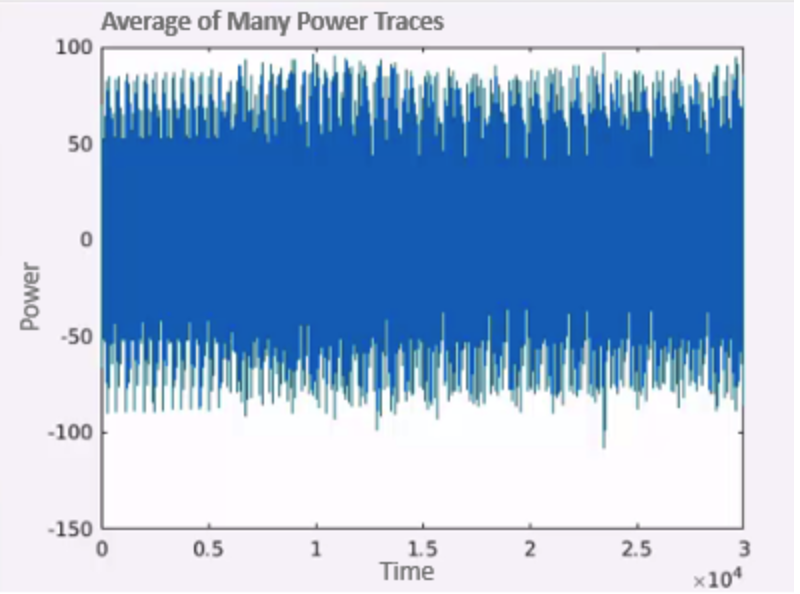
\includegraphics[width=0.8\textwidth]{images/Lecture6/avg_of_many_traces.png}
\caption{mean of each guess across the different inputs by time}
\label{fig:avg_of_many_traces}
\end{figure}
If we made the split correctly, this power trace average will be different from all the other 255 graphs.
The problem with this chart is that we need to check many graphs, so we need something that shows the distance of means for all the guesses.
A better graph will be to plot the distance of means of each key guess by time and then to search for the moment with the maximum difference ("the right time") like in figure: \ref{fig:intensity_represents_means_diff}
\begin{figure}[H]
\centering
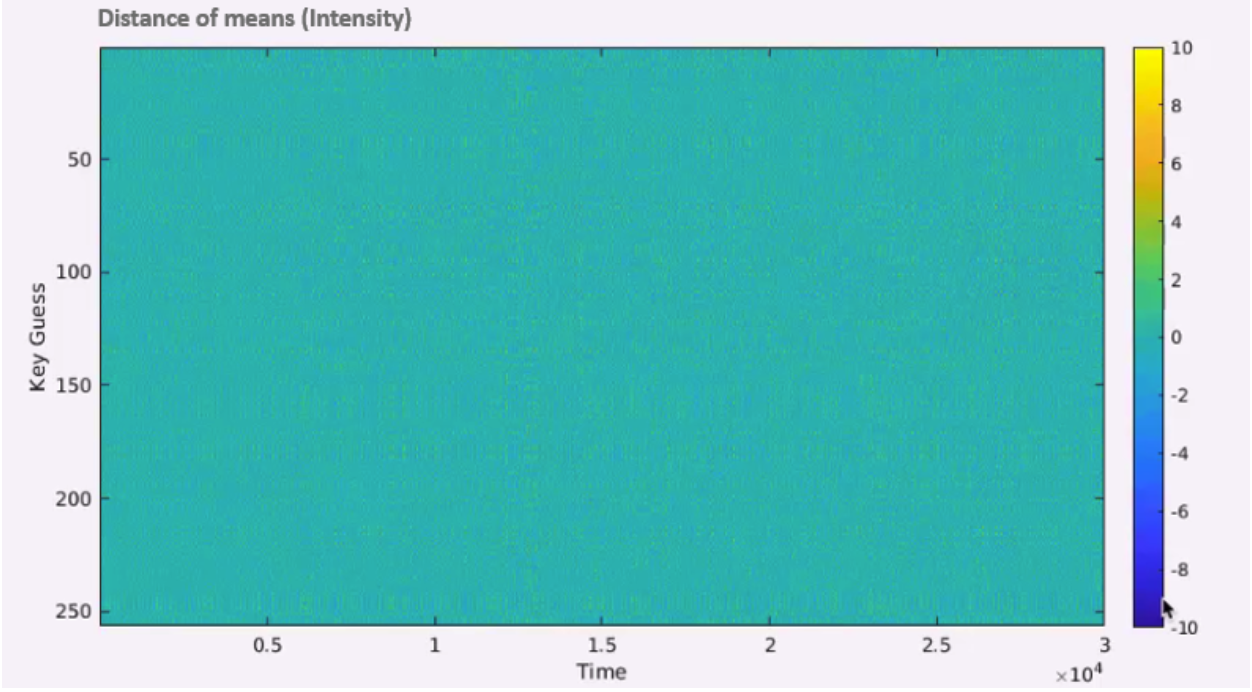
\includegraphics[width=0.8\textwidth]{images/Lecture6/intensity_represents_means_diff.png}
\caption{distance of means by time and key guess, color intensity represents the distance}
\label{fig:intensity_represents_means_diff}
\end{figure}
While it might be hard to spot it on this chart, there's a certain point of time where the difference is $8.91$, and at all the other points it's somewhere near 0 as we can see on the charts.

What if we focus on the correct time across the different key guesses? we should be able to spot the correct guess as shown in figure \ref{fig:the-correct-time}.
\begin{figure}[H]
\centering
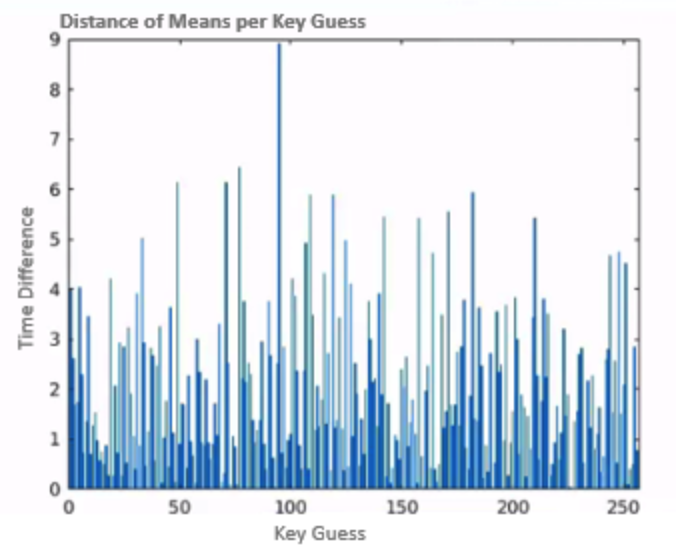
\includegraphics[width=0.8\textwidth]{images/Lecture6/the-correct-time.png}
\caption{means distance at the correct time}
\label{fig:the-correct-time}
\end{figure}

We finish by plotting the distance of means across time for all the keys, we can see in green the distance of means for the correct key and we can see that in the right time it's separated from the other keys as shown in figure \ref{fig:all}.
\begin{figure}[H]
\centering
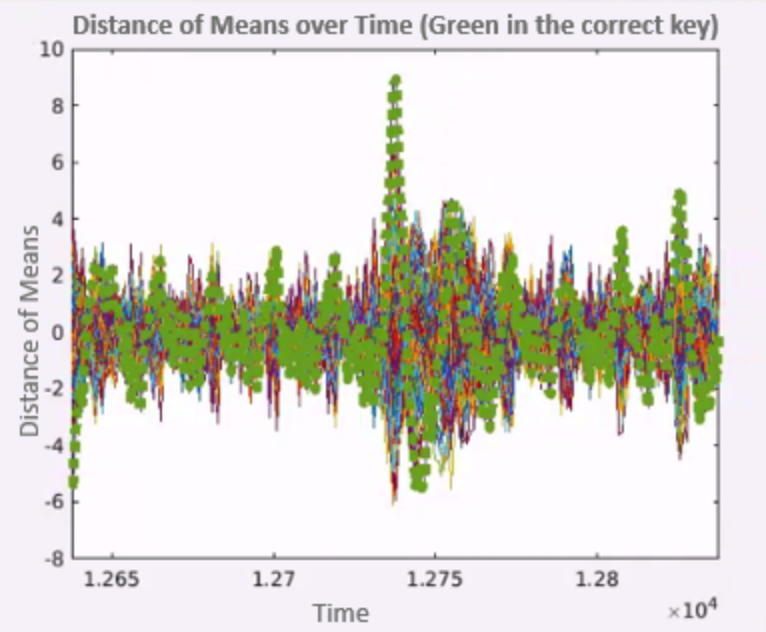
\includegraphics[width=0.8\textwidth]{images/Lecture6/all.png}
\caption{distance of means for all key guesses across time}
\label{fig:all}
\end{figure}


\chapter{Fault Attacks} \label{c9_ninthchapter:cha}

\begin{centering}
	\section*{Topics}
		\begin{enumerate}
			\begin{centering}
				\item Introduction to Fault Attacks
				\item Fault Attack on RSA-CRT
				\item DRAM and Rowhammer
				\item Flip-Feng-Shui: Rowhammer attack on RSA \\
			\end{centering}
		\end{enumerate}
\end{centering}
\newpage
\section*{Introduction to Fault Attacks}
Up until now in the course we learned about \emph{passive} attacks -- i.e. attacks which measure \emph{leakage} such as timing information and power traces. The advantage of these attacks is that they allow an attacker to acquire information in the process of an ongoing computation e.g. an AES key \emph{before} it was fully mixed with the input -- this fact can help the attacker extract secrets.

In fault attacks we will become \emph{active} in the sense that we will give the device-under-test (DUT) additional inputs such as heat or radiation.

One problem with Fault attacks: they use the strongest attack model, meaning -- we assume most power on the attacker's part.

\section{Active Attacks}
\paragraph{Definition:}
\begin{quote}
	\textit{"A fault attack is an active attack that allows extraction of secret information from cryptographic devices by breaking those devices."}
\end{quote}

In fault attacks we are being \emph{active} -- we give additional inputs beside the main input such as:
\begin{enumerate}
	\item Fuzzing (garbage or bad input)
	\item Radiation
	\item Heat
	\item Vibration
	\item Power spikes etc.
\end{enumerate}

This way, we receive other (usually erroneous) outputs which might give us additional information about the computation and/or the secret. This process is described in \cref{fig:fault_attacks_schematic}.

\begin{figure}[!ht]
	\centering
	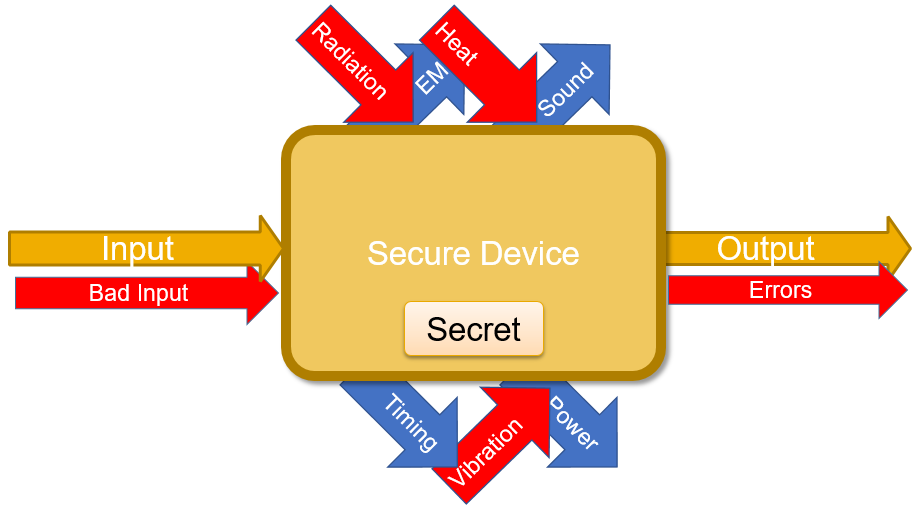
\includegraphics[width=0.7\linewidth]{images/ch9/fault_attacks_schematic.png}
	\caption{A schematic diagram of fault attacks and leakage types.}
	\label{fig:fault_attacks_schematic}
\end{figure}

Like with passive attacks, some of those outputs can be acquired at different stages of the computation process.

Many fault attacks are inspired by studies in the field of \emph{reliability}: a study in reliability will research a device's physical boundaries e.g. the maximum or minimum temperature under which it performs reliably. Other examples of reliability studies are aimed at improving device performance under extreme conditions such as:
\begin{itemize}
	\item Space and X-Rays
	\item Dense CPU Layouts
	\item Data Center Recovery (ECC-RAM)
\end{itemize}

A security researcher implementing fault attacks will, on the other hand,  purposefully subject the DUT to extreme conditions in order to inject errors in the device's functionality to achieve their goal. In that sense, a reliability study of a given device can lay the ground-work for the fault attacks to come.

\begin{quote}
	\textit{"In the reliability community things happen by mistake. In the security community -- things happen on purpose."}
\end{quote}

\subsubsection*{Breaking a device-under-test}
How can \emph{breaking} a device help an attacker?

\begin{enumerate}
	\item BORE -- \textit{"Break Once, Run Everywhere"}: Some device families share a single secret among all instances.
	\item Repairable Devices: Temporary breakage is fine. Sometimes restarting the device is enough to "repair" the damage.
	\item Partial breakage: Sometimes it's convenient to break \emph{part} of a device, for example -- destroy the subsystem responsible for DRM verification.
\end{enumerate}

\section{Fault Attack Taxonomy}
The tree ways we can examine a Fault Attack in order to understand it are:
\begin{enumerate}
	\item Method - \emph{"How to inject?"}
	\item Properties - \emph{"What fault to create?"}
	\item Target - \emph{"Which part to break?"}
\end{enumerate}

\subsection{Fault Methods}

\subsubsection{Power Supply Attacks}
What happens if the device is underpowered?
As we have previously seen, power in electronic devices is used to drive the CMOS transistors. If the device is slightly underpowered it might fail to switch some of the transistors and thus produce false calculations, and with even less power it might  struggle with getting into operational state (boot loop) or even transition to an entirely faulty state.
Another attack method involving the power supply is injecting power spikes (to a similar effect).

Some parts of a device are typically more sensitive to the power supply than others, and thus under- or over-powering the device will de-stabilize it and inject faults.

The obvious scenario for such an attack is when the DUT belongs to or is being controlled by the attacker -- for example if they're examining their own set-top box etc. In that case, the attacker can supply the device with as much/little power as they wish.

Another example of such attack scenarios is in the field of RFID readers -- the device powering an RFID chip is the reader, so a \emph{malicious} RFID reader can over/under-power the chip to achieve various faulty results.

\subsubsection{Clock/Timing Attacks}
The clock is typically a bus shared by many of the system's components which synchronizes the propagation of calculations through the system -- i.e. at the beginning all inputs are ready, and when there is a rising edge on the clock bus they start propagating throughout the various computational components. When all computations are finished they all wait for the next rising edge on the clock bus in order to proceed to the next stage.
In a clock glitching attack the attacker would inject a rising edge on the clock bus at an arbitrary time. This way only \emph{some} of the computations will have finished by that time while others are still being processed, and thus the device will be in a faulty (unstable) state.

A notable example is the attack on Mifare Classic RFID chips we talked about in the beginning of the course \cite{nohl2008} -- the RNG in the chip is only dependent on the time between powering up the RFID tag and challenging it. An RFID reader operated by the attacker can control both parameters, thus making the generated challenges deterministic.

\subsubsection{Temperature attacks}
This attack method relies on the physical property of electrons (current). Electrons  "jump", and the higher the temperature -- they will jump more frequently and to longer distances.
If a device gets \emph{too hot} -- enough electrons can "jump" e.g. over the insulation layer in a transistor to flip it from logical 1 to 0. This results in a fault.

Because of the ubiquity of devices failures due to temperature, nowadays temperature sensors are integrated into most devices, so when it overheats -- the device will shut down.

An attacker can bypass the temperature sensor by disconnecting it. Another method would be to quickly alternate the temperature of the device from extremely high to extremely low, so that \emph{on average} the temperature is reasonable, but it will still experience faults during the extreme phases of the cycles.

In an interesting research paper \cite{appel} a type-confusion attack on the Java virtual-machine was demonstrated: at first, the entire memory was filled with small arrays (say of size one). The Java VM is type-safe, so it is normally impossible to access one of the memory regions using a pointer to a different region. To inject a type-confusion fault the researchers used a 50W light bulb to heat the memory chip of the device enough to flip some of the bits (for illustration see \cref{fig:memory_lightbulb}). As a result, a small portion of the data-structures describing the arrays in memory now held wrong values (e.g. changed their value from $size=1$ to $size=20$). At this point, some affected data-structure \emph{contains} a header of a different data-structure, to which the attackers now have read and write access. Changing the header of the second data structure to an arbitrary value gave the attackers access to the entirety of the device's memory.
\begin{figure}[!ht]
	\centering
	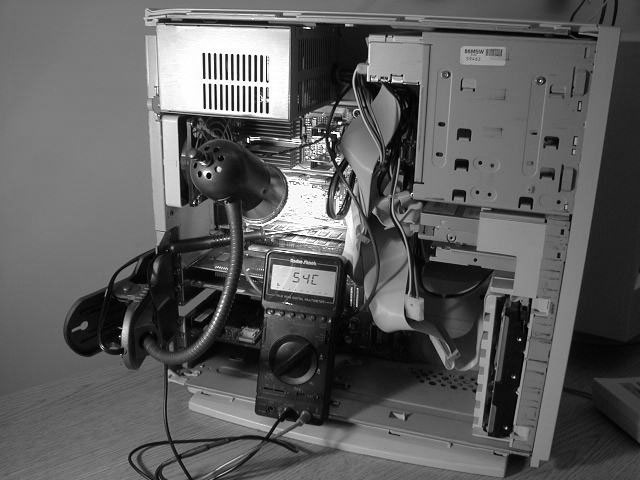
\includegraphics[width=0.7\linewidth]{images/ch9/bulb.png}
	\caption{A light bulb flipping memory bits filled with safe Java structures.}
	\label{fig:memory_lightbulb}
\end{figure}

\subsubsection{Optical, Electromagnetic}
When a laser hits a transistor it changes the energy level of the silicon inside, and sometimes it can change the transistor's state. Notably different wavelengths are absorbed by different materials, so in a typical silicon chip different lasers will hit different layers of the device etc. Magnetic/Electromagnetic radiation and pulses have similar effects.

The underlying principal of those attacks is that the attacker forcefully injects charge (energy) into the device. Once it's stored inside it will have to dissipate one way or another, so as a result it injects a random faulty state into the device.

\subsubsection{Reading from RAM}
All of the attacks described above require very high engagement with the DUT -- in order for the attacker to control the power/clock sources, for example, they sometimes would need to drill, cut or otherwise tamper with the device. Shining a laser on a device requires at the very least having it at a visible distance.

The final attack method involves only \emph{reading} from memory, and thus is very practical and requires very little physical engagement. This attack method is called \emph{Rowhammer} and is discussed later in the lecture.


\subsection{Fault Properties}
In this section we discuss:
\begin{enumerate}
	\item How controllable is the fault's location/size? Precise? Loose? None?
	\item How controllable is the fault timing?
	% Can we have the fault occur when something exciting is happening?
	% Heat is the LEAST controllable -- it's a gradual and stochastic process. Freaking Lasers -- very controllable.
	\item What's the fault's duration? Transient? Permanent? Destructive?
\end{enumerate}


\subsubsection*{Destructive fault attacks on cryptographic devices}
What can be done with fault attacks to symmetric ciphers?
\paragraph{Easy example:} Imagine that we have a pile of cipher devices with a 64bit key length, which work the following way: we can give the device a key and it tells us whether it's the right key.

What if we have a DESTRUCTIVE fault attack that resets the top 32bits of a device's key? We can brute force the key in $2\cdot2^{31}$ instead of $2^{63}$ (on average):

First we inject the fault into one of the devices and brute-force the lower 32 bits of the key ($O(2^{31})$), then we pick another device from the pile and brute-force only the higher 32 bits (another $O(2^{31})$).

\paragraph{A less trivial example:} We have a public-key device which we can ZAP and one bit of the key flips to zero.

We can save all of the plaintexts-cipher pairs until we reach the one matching an all zero key -- which we can pre-calculate. This gives us the Hamming weight of the key.
Now we go back one plaintext-cipher pair -- we know that pair's key's Hamming weight to be exactly one -- meaning we need to brute-force only $N$ keys ($N$ is the key bit-length). Now we have the position of a single bit of the key.

If we iterate all the way backwards to the original plaintext-cipher pair, we can acquire the key in $O(N^2)$ time!

\subsection{Fault Target}
What could be targeted by a fault attack?
\begin{enumerate}
	\item Input parameters (fuzzing, clock glitching)
	\item Storage (volatile/non-volatile)
	\begin{enumerate}
		\item HDD - Destructive (persists after reset)
		\item RAM - Permanent
		\item Cache - Transient
	\end{enumerate}
	% If we fault the disk/flash? It's a destructive fault! If we fault the RAM, the fault is permanent (not destructive). In cache? Transient fault!
	% What other storage is there? Instruction cache.
	\item Data processing: inject a fault mid-computation and the device gives a different answer.
	\item Instruction Processing/Control Flow: inject a fault in the IP register and change the instruction flow.
	\begin{enumerate}
		\item ARM32 instructions are very densely packed, thus there is a very high probability of hitting a valid instruction after flipping a single bit. \texttt{jnz} and \texttt{jmp} are only one bit apart.
		\item Change for loop condition to dump RAM contents including source code.
	\end{enumerate}
\end{enumerate}

\paragraph{Two examples of Fault Attacks targeting Control Flow:}
\begin{enumerate}
	\item The CHDK hacking community, used to dump the firmwares of Canon cameras via blinking one of their LEDs \cite{chdk, bib:canon}.

	\item "The Unlooper": Back in the 90's pay-tv devices started cryptographically signing the content, and if the cryptographic checksum did not check out -- the device would enter an endless loop. The hacking community invented "unloopers" -- a gadget that would inject a power spike and fault the IP register, so that the pay-tv device would jump to some other section of the code, from which point it would function normally.
\end{enumerate}

\section{Fault attack on RSA-CRT}

\subsection{RSA decryption}
\[
	N = p\cdot q
\]
\[
	M = C^d (mod\ n) = M^{ed} (mod\ n) = M^1 (mod\ n)
\]

RSA decryption is hard!

Let's speed it up using CRT (the Chinese Remainder Theorem):
Multiplication operations are $O(|n|^2)$. If we can do operations $(mod\ p)$ and then $(mod\ q)$ instead of $(mod\ n)$, we will reduce computation time by half.

\paragraph{Explanation:}

The bit-lengths of $p$ and $q$ are each half that of $n$
\[|p|=|q|=\frac{1}{2}|n|\]
The computational complexity of multiplying by a number of length $x$ is (roughly) $O(x^2)$. Thus:
\[
O(|p|^2) = O(|q|^2) = \frac{1}{4}O(|n|^2) \Rightarrow (O(|p|^2) + O(|q|^2)) = \frac{1}{2}O(|n|^2)
\]

So if we could multiply by $p$ and $q$ instead of by $n$, we would cut \emph{each} multiplication operation's time complexity in half!

\subsubsection{Chinese Remainder Theorem}
\begin{figure}[!ht]
	\centering
	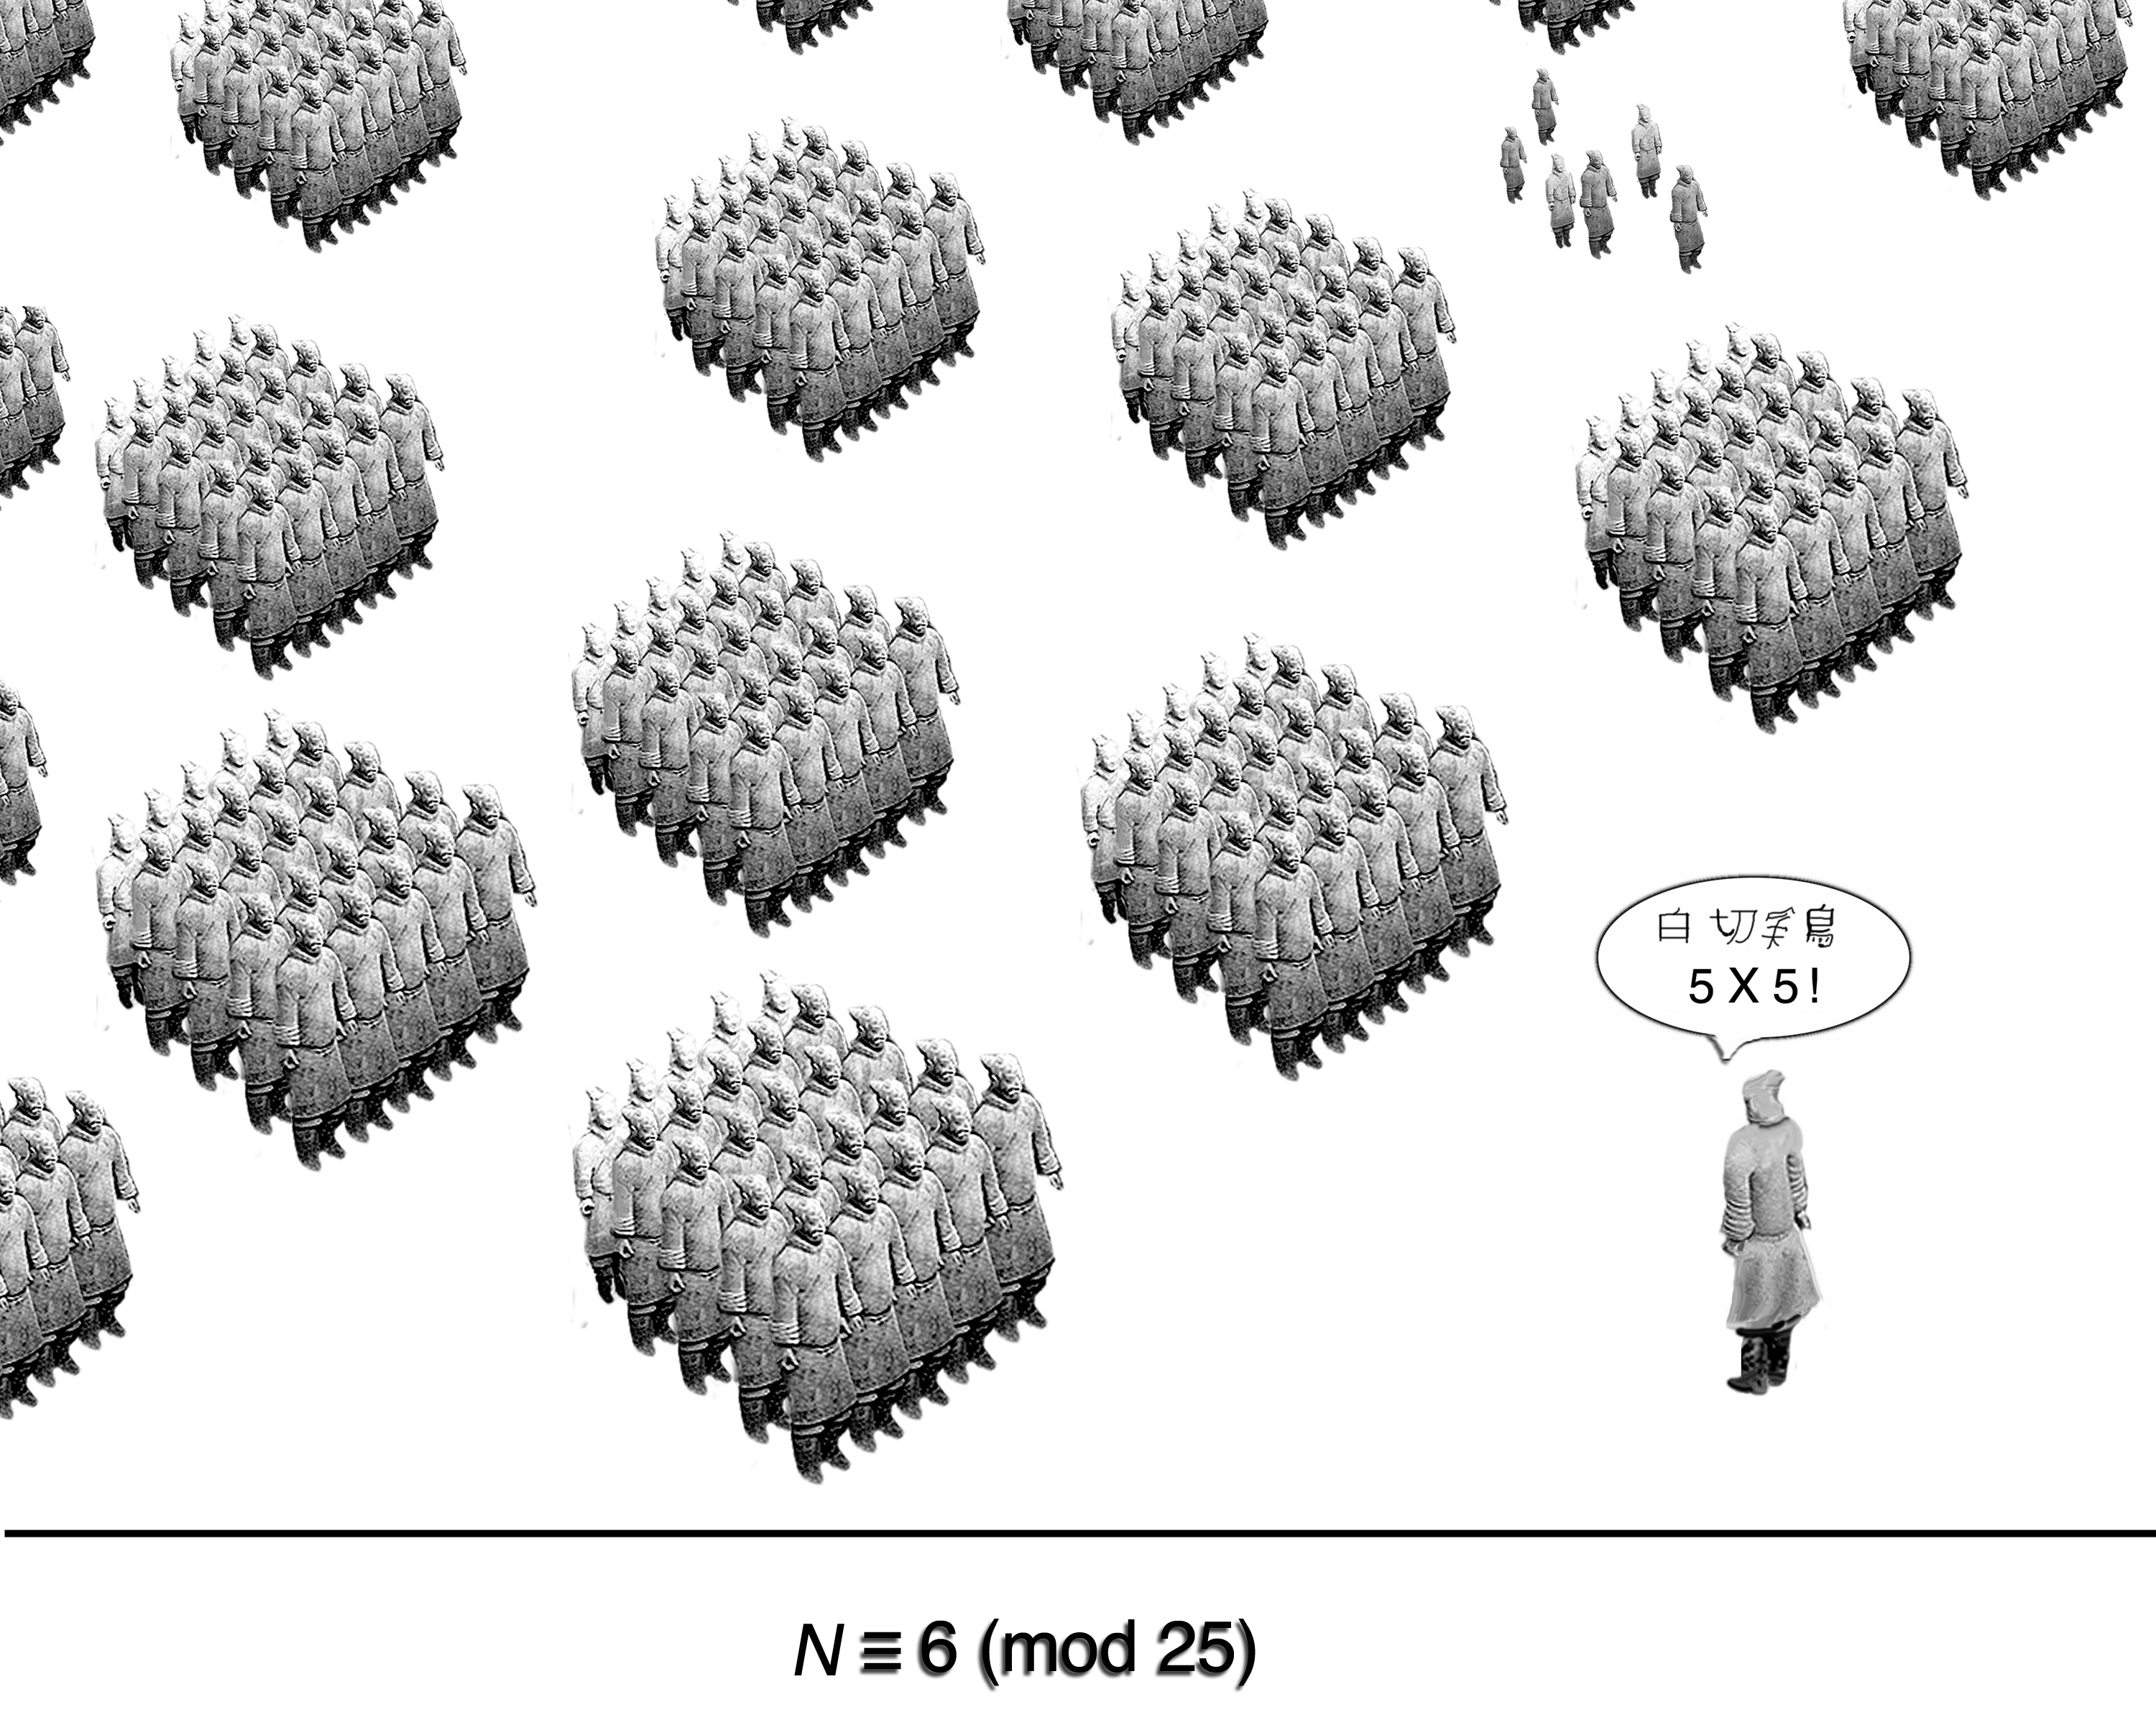
\includegraphics[width=0.5\linewidth]{images/ch9/soldiers.jpeg}
	\caption{Chinese Remainder Theorem (Source: \url{https://russinoff.com/papers/crt.html})}
	\label{fig:chinese_remainder}
\end{figure}
The idea is that if we know both $x (mod\ p)$ and $x (mod\ q)$ then we can easily calculate $x (mod\ n)$.

So, given a message $M$ calculate $M_p$ and $M_q$:
\[M_p = C^d (mod\ n)(mod\ p) = C^d (mod\ p)\]
\[M_q = C^d (mod\ n)(mod\ q) = C^d (mod\ q)\]

To combine the values, we do:
\[
	M^* = CRT(M_p, M_q) = M_p \cdot q \cdot (q^{-1} mod\ p) + M_q \cdot p \cdot (p^{-1} mod\ q)
\]

It is easily provable that \(M^*(mod\ p)=M_q\) and \(M^*(mod\ q)=M_p\), so by the Chinese Remainder Theorem, this value \emph{must} be equal to $M$.

\subsubsection{The Boneh, DeMillo \& Lipton Fault Attack on RSA-CRT \cite{boneh}}

The attacker has a decryption box (known plaintext scenario) with public key $n$ and would like to recover $d$ (the private key). Additionally, the attacker knows that the decryption box is decrypting using CRT. Finally, let us assume that the attacker can inject a fault (any fault) in the decryption process.

The attacker first gets \(M = M_p*q*(q^{-1} mod\ p) + M_q*p*(p^{-1} mod\ q)\)
through the regular decryption process.

Then, the attacker primes the device to re-calculate the message from the same cipher, this time injecting a \emph{fault} during the calculation of $M_p$, resulting in the device erroneously producing $M'_p$ instead:
\[M'_p \neq C^d (mod\ p)\]
The device will then proceed to combine $M'_p$ with the correct result of $M_q$, resulting in:
\[M' =  M'_p \cdot q \cdot (q^{-1} mod\ p) + M_q \cdot p \cdot (p^{-1} mod\ q)\]

Now the attacker can calculate the value of $M - M'$:
\[
	 (M_p \cdot q \cdot (q^{-1} mod\ p) + M_q \cdot p \cdot (p^{-1} mod\ q)) - (M'_p \cdot q \cdot (q^{-1} mod\ p) + M_q \cdot p \cdot (p^{-1} mod\ q)) =
\]
\[
	(M_p - M'_p) \cdot q \cdot (q^{-1} mod\ p))
\]

Finally, calculating the $gcd$ of $n$ and $M - M'$ yields:
\[
	\gcd(n, M - M') = \gcd(p \cdot q, (M_p - M'_p) \cdot q \cdot (q^{-1} mod\ p)) = q
\]

\paragraph{Why does this work?} The greatest common divisor of $n$ and anything can be only $p$, $q$, $n$ or $1$. On the other hand, $M_p$ and $M'_p$ can never be multiples of $p$, otherwise both would equal 0. So, by that reasoning, $\gcd(p \cdot q, (M_p - M'_p) \cdot q \cdot (q^{-1} mod\ p))$ \underline{must} equal $q$, and thus we have cracked the cipher using a single fault attack.

A later paper co-written by Arjen Lenstra \cite{lenstra} further improved upon this attack to not require knowledge of $M$.

\paragraph{BML in practice:} A paper \cite{schmidt} showed how ZAPPING a device with an electric spark from a lighter during computation can achieve the described effect.

\section{Rowhammer}
In the final section, we will describe the Rowhammer attack.
\subsection{Rowhammer attack taxonomy}
	\begin{itemize}
		\item Target: DRAM on modern computers
		\item Properties: Permanent, controlled location
		\item Method: Memory accesses
	\end{itemize}

\begin{figure}[!ht]
	\centering
	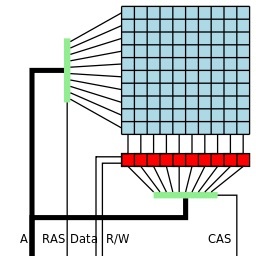
\includegraphics[width=0.5\linewidth]{images/ch9/DRAM.jpg}
	\caption{High Level Illustration of DRAM Organization (Source: Wikipedia:Row Hammer)}
	\label{fig:dram_svg}
\end{figure}

\subsection{Double-sided Rowhammer}
DRAM is the most common type of volatile memory. It is slow, dense and cheap relatively to SRAM. Every bit of RAM is stored in a single capacitor.

The attack \cite{rowhammer} utilizes the physical structure of RAM chips in order to induce faults: Due to parasitic leakage in DRAM capacitors, if enough consecutive reads are performed on the immediately adjacent rows eventually a bit will flip in the target row.

\subsubsection{The challenge of CPU caching}
The CPU cache prevents the same memory address to be read consecutively from main memory, for performance reasons.
To circumvent this limitation, several techniques can be employed:
\begin{enumerate}
	\item Intel CPUs provide non-temporal read/write opcodes -- special instructions that read from memory and don't get cached.
	\item The special \texttt{clflush} instruction can be used to explicitly flush the cache after each read operation (privileged operation).
	\item Finally, cache-population algorithms had been extensively studied and reverse-engineered, so it is possible to arrange for \emph{arbitrary} cache misses.
\end{enumerate}

\subsection{Countermeasures}
\paragraph{Refresh-rate increase:} In order to overcome parasitic leakage, DRAM chips already have a mechanism in place to read and then re-write the values stored in each row periodically. One method of overcoming Rowhammer could be to significantly increase the refresh-rate of the chip. This obviously results in both performance degradation and increased power consumption.

\paragraph{ECC-RAM:} High-end DRAM chips (typically meant for data center environments) contain error-correction coding (ECC) logic which can typically \emph{correct} one erroneous bit and \emph{detect} two (at which point it will crash the program/system). Those chips are immune to the basic form of Rowhammer described above, but as discussed later, are not bullet-proof.

\subsection{Rowhammer variations}
\subsubsection{Flip Feng-Shui}
\paragraph{Page de-duplication:} On modern systems, typically much memory is shared among many processes running on the system. This is even more true of virtualized environments where the guest and the host, for example, could run the same OS. A common optimization is for the system to detect and de-duplicate pages containing the same data, thus freeing up memory.
\paragraph{Rowhammer + page de-duplication:}
In a paper \cite{ffs} researchers from VUA demonstrated how they can utilize page-deduplication in a virtualized environment to weaken cryptographic keys, resulting in unauthorized access via OpenSSH, and breach of trust via forging GPG signatures. The attack relies on the fact that the the attacker can \emph{read} a de-duplicated page as much as they want. The attacker has to wait (or arrange) for a page containing sensitive information to be de-duped, then hammer on it until a bit in the key flips, making it much easier to factor.
\begin{figure}[!ht]
	\centering
	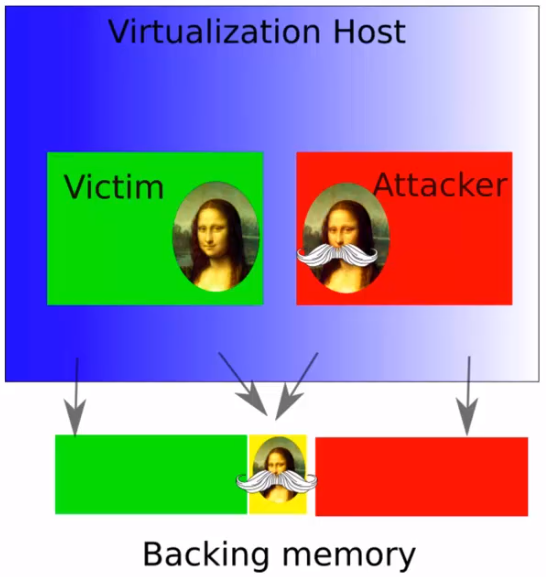
\includegraphics[width=0.5\linewidth]{images/ch9/flip_feng_shui.PNG}
	\caption{The attacker maps the same page as the victim, then utilizes rowhammer to change the victim's memory without causing page duplication.}
	\label{fig:flip_feng_shui}
\end{figure}

\subsubsection{ECCPloit}
In another paper \cite{eccploit} researchers from VUA showed how they can use Rowhammer to quickly flip \emph{enough} (typically three) bits on an ECC-RAM chip that error correction will not be able to detect it, thus defeating the ECC mitigation. The attack relies on the fact that error-correction takes time to compute, and this gives the attacker a window of opportunity.


\clearpage
\bibliographystyle{unsrt}
\bibliography{bibliography/english}

\end{document}
